% !TEX root = main.tex
\chapter{Data sample and selection}

This analysis is done on the data sample recorded by the \lhcb experiment in \num{2011} and \num{2012} at centre-of-mass energies of \SI{7}{\tera\electronvolt} and \SI{8}{\tera\electronvolt}, respectively.
In \num{2011} the detector collected \SI{1}{\per\femto\barn}, while in \num{2012} \SI{2}{\per\femto\barn} were collected.
In this chapter the used data samples as well as the simulated samples are described (\cref{sec:Samples}).
Following, the selection procedure is reported, divided into preselection and trigger requirements (\cref{sec:preselTrigger}), vetoes for \eg misidentified background events (\cref{sec:vetoes}) and a multivariate classifier to reduce combinatorial background (\cref{sec:MVADev} and \cref{sec:BDTOpt}).
Last the handling of multiple $B$-candidates in one event is presented (\cref{sec:MultCands}) and the selection performance is given (\cref{sec:selectionPerformance}).

\section{Data and simulation samples}
\label{sec:Samples}

Candidates for the decay \BdToDpi are reconstructed in the hadronic decay $\Dpm\!\to\Kmp\pipm\pipm$ with one additional pion, which will be denoted as bachelor pion in the following.
Since the \D-decay is the one with the largest decay width it is chosen, despite the purely hadronic final state.
It is reconstructed inclusively, \ie no resonances as the decay via a \Kstarz are excluded.
For several tests and crosschecks the datasample can be split by year of data taking (\num{2011} and \num{2012}) and magnet polarity (up and down).

To distinguish the charged hadrons in the finalstate a likelihood function assuming the respective particle to be a pion or a kaon is computed for every particle using information from the PID system.
Then the difference between the two logarithmic likelihoods is calculated, in the following referred to as \dllkpi.
To identify other particles like protons a likelihood function assuming the corresponding hypothesis can be computed and compared in the same way with the pion hypothesis.
Using the \dllkpi of the bachelor pion allows to split the data sample in two parts: The first sample denoted as \emph{pion}-sample with $\dllkpi\leq5.0$ and a second sample denoted as \emph{kaon}-sample with $\dllkpi>5.0$. This distinction is useful when separating \BdToDpi from $\Bd\!\to\Dm\Kp$ candidates as no dedicated selection cut is needed
Instead this separation can be done statistically in the fit to the invariant mass distribution (see \cref{ch:massfit}).

The simulated samples used in this analysis are listed in \cref{tab:simSamples}, together with short reference in which step they are needed\footnote{charge conjugation is implied throughout the whole document if not stated otherwise}.
\begin{table}[tbp]
	\centering
	\caption{Simulated samples used in this analysis with a short note in which analysis step the samples are used.
	Charged \D-mesons are always generated with the decay $\Dm\!\to\Kp\pim\pim$, uncharged \D-mesons with the decay $\Dzb\!\to\Kp\pim$.}
	\begin{tabular}{lc}
		\toprule
		sample & analysis step \\
		\midrule
		$\Bz\!\to\Dpm\pimp$ 														& selection, massfit, flavour tagging, time fit \\
		$\Bs\!\to\Dsm\!\left(\to\Kp\Kp\pim\right)\pip$  							& selection \\
		$\Lb\!\to\Lcbar\!\left(\to\Kp\antiproton\pim\right)\pip$ 					& selection \\
		$\Bz\!\to\Dm\Kp$ 															& massfit \\
		$\Bz\!\to\Dm\rhop\!\left(\to\pip\piz\!\left(\to\g\g\right)\right)$ 			& massfit \\
		$\Bz\!\to\Dstarm\!\left(\to\Dm\piz\right)\pip$ 								& massfit \\
		$\Bz\!\to\Dm\Kstarp\!\left(\to\Kp\piz\right)$ 								& massfit \\
		$\Bz\!\to\jpsi\!\left(\to\mup\mun\right)\Kstarz\!\left(\to\Kp\pim\right)$ 	& flavour tagging \\
		$\Bu\!\to\Dzb\pip$ 															& flavour tagging \\
		$\Bu\!\to\Dzb\Kstarp\!\left(\to\Kp\pim\right)$ 								& flavour tagging \\
		$\Bu\!\to\Dstarb\!\left(\to\Dz\g\right)\pip$ 								& flavour tagging \\
		$\Bu\!\to\Dzb\Kstarp\!\left(\to\Kp\piz\right)$ 								& flavour tagging \\
		$\Bz\!\to\Dzb\pip\pim$ 														& flavour tagging \\
		\bottomrule
	\end{tabular}
	\label{tab:simSamples}
\end{table}
As the PID observables are not described well in the simulation selection requirements on such observables can result in different distributions in other, correlated observables.
Moreover efficiencies of PID requirements will be wrongly described in the simulation, what would lead to mistakes in the handling of the \emph{pion}- and \emph{kaon}-sample in the massfit, described in \cref{ch:massfit}.
Therefore the \dllkpi and \dllppi variables are corrected using calibration samples of kinematically-clean $\Dstar\!\to\Dz\!\left(\to\Km\pip\right)\pip$ decays.
The correction is done in bins of transverse momentum \pt and pseudorapidity $\eta$.
For every candidate in the simulation the corresponding PID distribution of the calibration sample in the $(\pt,\eta)$-bin is built and used to randomly sample a PID value.

Last, to obtain the correct correlations and uncertainties between vertex positions, particle momenta, decay times and invariant masses decay tree fits (DTF) are performed on the data and simulations~\cite{2005NIMPA}.
In total, three DTFs are performed: To determine observables correlated with the decay time, the \ac{PV} is constrained to the known point of the proton-proton collision.
Observables correlated to the invariant mass stem from a DTF where the mass of the \Dm-meson is constrained to its known mass of $m_\Dm^{\text{PDG}}=\SI[per-mode=symbol]{1869.61}{\MeVcc}$~\cite{PDG_2017}.
A third DTF is performed without any constraint, as for selection steps like optimising the vetoes described in \cref{sec:vetoes}, constraints would lead to wrong results.

\section{Selection}
\label{sec:selection}

As a first step, the so-called stripping is applied to the \BdToDpi candidates with \mbox{$\Dpm\!\to\Kmp\pipm\pipm$}.
The stripping is a first loose preselection common to a set of kinematically similar decays.
Events with more than \num{500} tracks, which are constructed from hits in the \velo and the tracking stations T1 to T3, are rejected.
The criteria on the charged tracks are partially different whether the charged track is considered as the bachelor particle, or as a \Dm daughter.
Three of these charged tracks are then used to form a \Dm-meson, where the (transverse) momentum of one of the three tracks has to exceed (\SI[per-mode=symbol]{500}{\MeVc}) \SI[per-mode=symbol]{5}{\GeVc} and its track $\nicefrac{\chi^2}{\text{ndof}}$ has to be less than \num{2.5}.
This \Dm-meson is then combined with a charged bachelor track to form a \Bz-meson.
Finally a bagged boosted decision tree trained on simulation is applied, and its response is required to be larger than \num{0.05}.
All requirements on single particles are given in \cref{tab:stripping}.
\begin{table}[tbp]
	\centering
	\caption{Stripping cuts for the decay \BdToDpi with $\Dpm\!\to\Kmp\pipm\pipm$.
	For the charged tracks the more stringent requirements for the bachelor track are given in brackets.
	The decay vertex of the \Bz-meson is denoted as \ac{SV}, for the impact parameter the shortcut IP is used and the distance of closest appraoch of the \Dm daughter particles w.r.t. each other is denoted as DOCA.}
	\begin{tabular}{cc}
		\toprule
		\multicolumn{2}{c}{charged tracks requirements}\\
		\midrule
		track $\nicefrac{\chi^2}{\text{ndof}}$		& $<3.0 (2.5)$ \\
		momentum $p$ 								& $>\SI[per-mode=symbol, separate-uncertainty=false]{1\pm5}{\GeVc}$ \\
		transverse momentum \pt 					& $>\SI[per-mode=symbol, separate-uncertainty=false]{100\pm500}{\MeVc}$ \\
		IP $\chi^2$ w.r.t. any \ac{PV}				& $>4.0$ \\
		track ghost probability 					& $<0.4$ \\
		\midrule
		\multicolumn{2}{c}{\Dm-meson requirements}\\
		\midrule
		$\sum \pt\left(hhh\right)$ 																				& $>\SI[per-mode=symbol]{1800}{\MeVc}$ \\
		DOCA 																									& $<\SI{0.5}{\milli\metre}$ \\
		$m_\Dm$ 																								& \SIrange[per-mode=symbol,range-units=single]{1769.92}{2068.49}{\MeVcc} \\
		\ac{SV} $\nicefrac{chi^2}{\text{ndof}}$ 																	& $<10.0$ \\
		vertex separation $\chi^2$ to any \ac{PV} 																	& $>36.0$ \\
		$\cos$ of $\sphericalangle\left[\left|\text{PV},\Dm\text{-Vtx}\right|, \vec{p}\!\left(\Dm\right)\right]$	& $>0.0$ \\
		\midrule
		\multicolumn{2}{c}{\Bz-meson requirements}\\
		\midrule
		\ac{SV} $\nicefrac{\chi^2}{\text{ndof}}$ 																& $<10.0$ \\
		reconstructed decay time $t$ 																			& $>\SI{0.2}{\pico\second}$ \\
		IP $\chi^2$ w.r.t. the associated \ac{PV} 																& $<25.0$ \\
		$\cos$ of $\sphericalangle\left[\left|\text{PV},\text{SV}\right|, \vec{p}\!\left(\Bz\right)\right]$		& $>0.999$ \\
		\bottomrule
	\end{tabular}
	\label{tab:stripping}
\end{table}
Following the stripping, a decay-specific selection described in the following sections is applied.

\subsection{Preselection and trigger requirements}
\label{sec:preselTrigger}

Before applying further selection requirements to reduce the background, requirements on the trigger are made.
In principle there are two different classes of trigger decisions at \lhcb: A trigger can fire due to a particle or event property directly connected to the signal decay - denoted as trigger on signal (TOS) - or it can fire due to some property separate to the signal decay what is denoted as a decision independent of the signal (TIS).
Furthermore, each trigger stage has various lines, triggering on different event properties and thus being differently effective depending on the specific decay.
Hence, a requirement on which trigger line has fired and whether this decision is TOS or TIS results in characteristic distribution of observables such that a decision which requirement is made needs to be done analysis specific.

\begin{figure}[tbp]
    \centering
    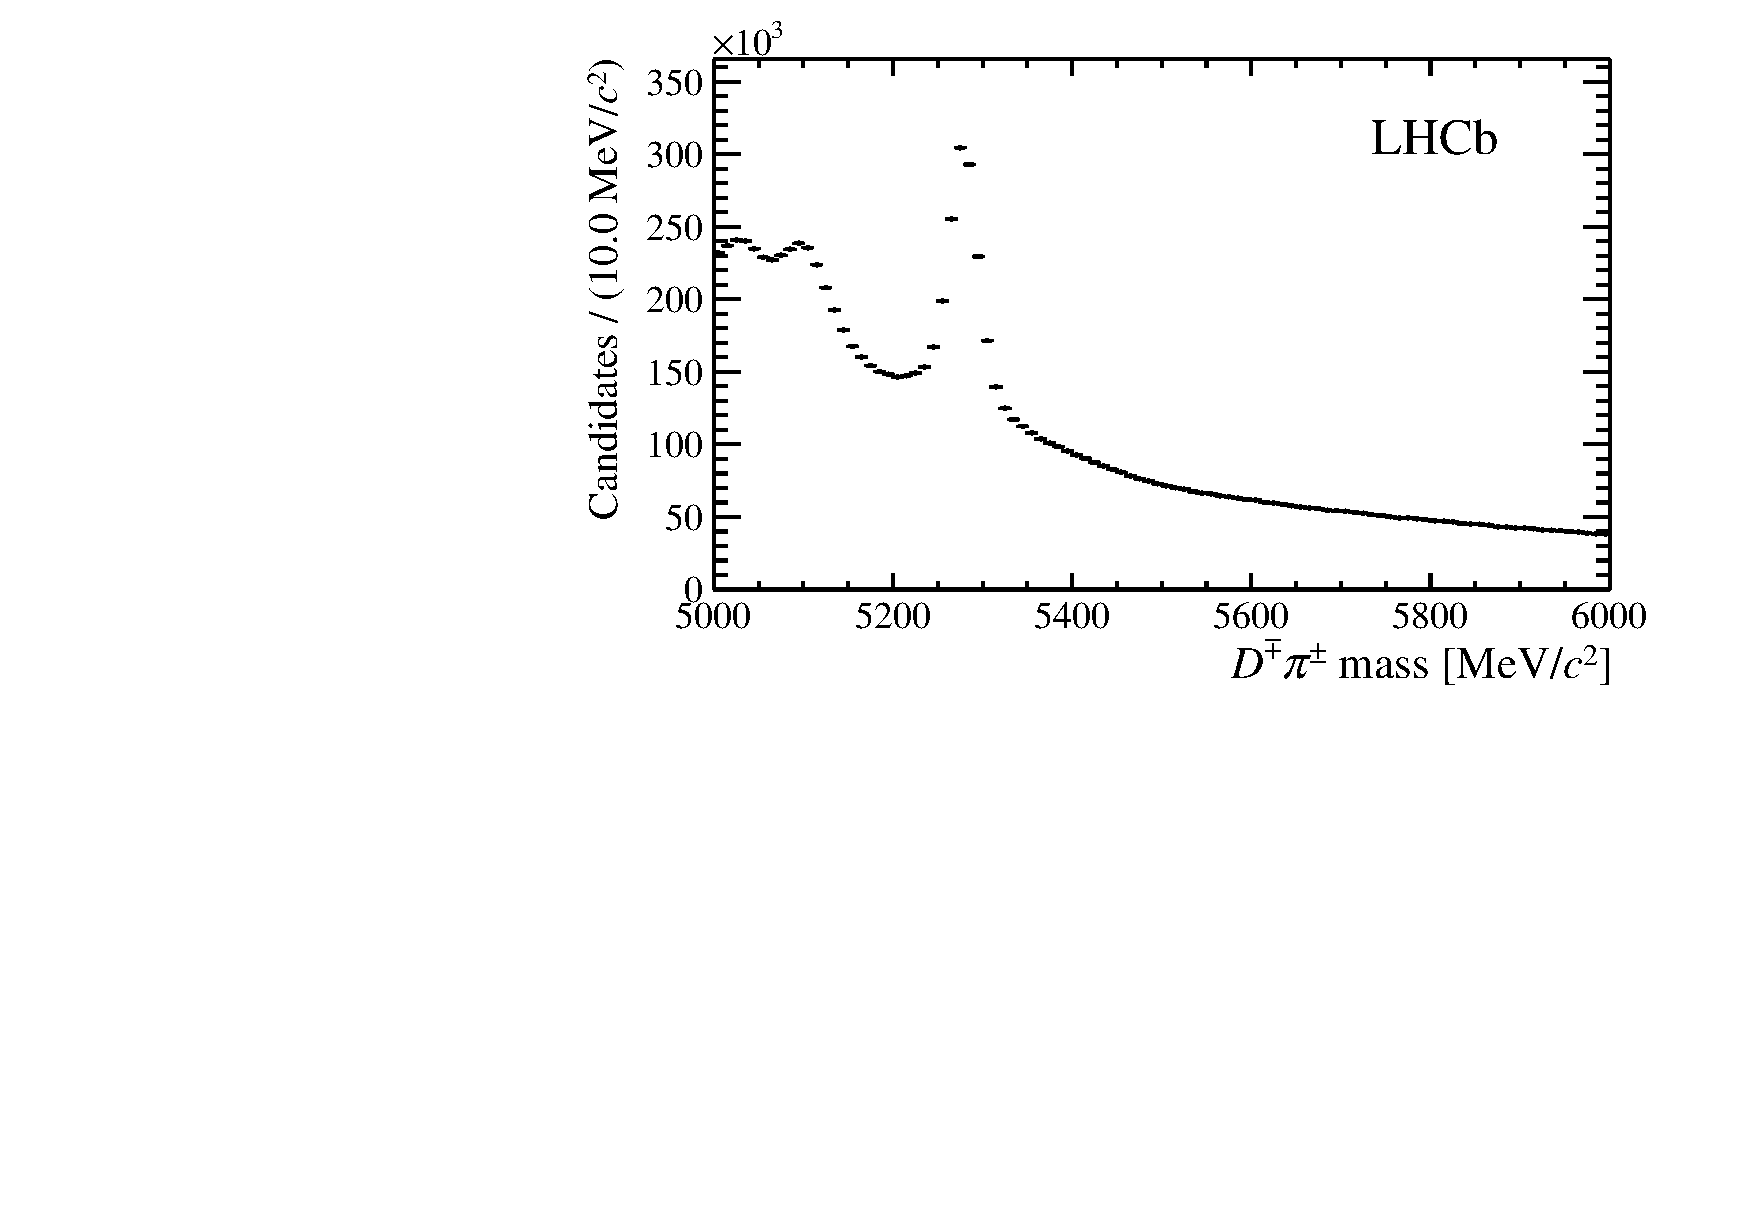
\includegraphics[width=0.49\textwidth]{06selection/figs/Bmass_afterStrippingAndTrigger.pdf}
    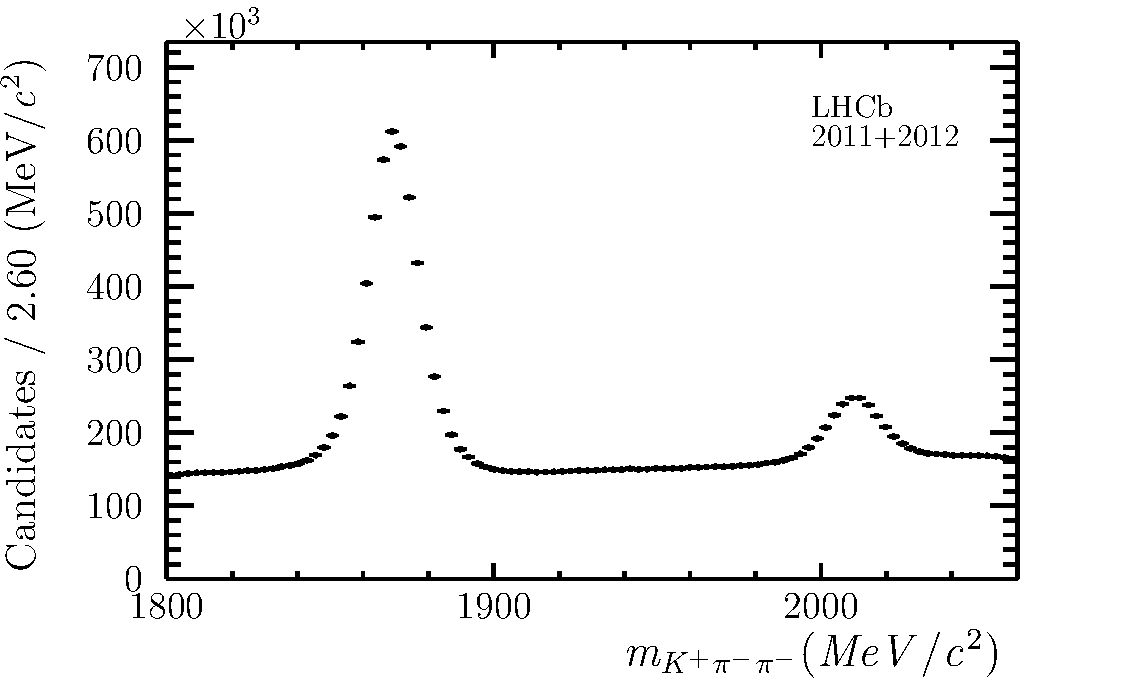
\includegraphics[width=0.49\textwidth]{06selection/figs/Dmass_afterStrippingAndTrigger.pdf}
    \caption{Invariant mass distributions of the $\Dm\pip$ combination using the DTF with a \Dm-mass constraint (right) and of the \Kp\pim\pim combination without any constraint (right).}
    \label{fig:BAndDmassAfterStripping}
\end{figure}
For this analysis no specifc requirements at the L0 level are made.
On the HLT1 level the \Bz candidates are required to be TOS on the \verb!Hlt1TrackAllL0Decision! line
In the HLT2 trigger stage the \BdToDpi candidates are required to be TOS on either the \verb!Hlt2Topo2BodyBBDTDecision! line, the \verb!Hlt2Topo3BodyBBDTDecision! line  or the \verb!Hlt2Topo4BodyBBDTDecision! line.
These lines require a \ac{SV} formed out of two, three or four tracks with a significant separation from the \ac{PV}~\cite{Trigger_Gligorov}.
In \cref{fig:BAndDmassAfterStripping} the invariant mass distributions of the \Bz and \Dm candidates are shown. The \Bz peak is clearly together with structures from the partially reconstructed decays $\Bz\!\to\Dm\rhop$ and $\Bz\!\to\Dstarm\pip$.
The distribution of the invariant mass of the \D-meson shows the \Dm peak at \SI[per-mode=symbol]{1870}{\MeVcc} and a \Dstarm peak at \SI[per-mode=symbol]{2010}{\MeVcc}.
After the trigger requirements some lose sanity cuts to remove clear background candidates are applied.
These cuts are listed in \cref{tab:preselection}.
\begin{table}[tbp]
	\centering
	\caption{Preselection cuts applied after the trigger requirements.}
	\begin{tabular}{cc}
		\toprule
		\multicolumn{2}{c}{\Dm daughter requirements}\\
		\midrule
		\dllkpi for pions	& $<8.0$ \\
		\dllkpi for kaons 	& $>-2.0$ \\
		\midrule
		\multicolumn{2}{c}{\Dm- and \Bz-meson requirements}\\
		\midrule
		$\left|m_{\Kp\pim\pim}-m_\Dm^{\text{PDG}}\right|$	& $<\SI[per-mode=symbol]{35}{\MeVcc}$ \\
		\Bz decay time										& $>\SI{0.2}{\pico\second}$ \\
		\bottomrule
	\end{tabular}
	\label{tab:preselection}
\end{table}

\subsection{Vetoes}
\label{sec:vetoes}

Before a multivariate classifier is trained on and applied to a data sample, this should at best only consist of the candidates which are supposed be separated by the classifier.
In this case these candidates are \BdToDpi signal candidates and combinatorial background.
Therefore backgrounds due to kinematic failures in the reconstruction and wrong associations between a \Bz candidate and a \ac{PV} are vetoed.

\subsubsection*{Mass vetoes}

First, the investigated sources of backgrounds which arise due to failures in the reconstrucion, and if necessary, the applied vetoes are described.
Such failures can be missed neutral particles or misidentified particles in the reconstruction.

The first type of backgrounds arises from the decay $\Bz\!\to\Dm\mup\neum$. When missing the neutrino and misidentifying the muon as a pion this decay would falsely be reconstructed as the signal decay \BdToDpi.
This is vetoed with a binary requirement on the bachelor particle not to be a muon.
This binary requirement is based on the number and the region of the muon stations where hits are found and the momentum of the track~\cite{Archilli:2013npa}.

The following kinematic backgrounds are all due to misidentification of particles in the finalstate.
Misidentification between protons and pions can lead to backgrounds from $\Lb\!\to\Lcbar\pip$ decays where the \Lcbar decays into a kaon, a pion and an antiproton.
To identify such background candidates a proton-mass hypothesis is applied to both daughter pions of the \Dm-meson.
After combining the three \D daughters again a peak around the \Lc mass becomes visible in the distributions shown in \cref{fig:LcVeto}.
The distributions look different, because of the pions, which are originally sorted by transverse momentum \pt.
\begin{figure}[tbp]
    \centering
    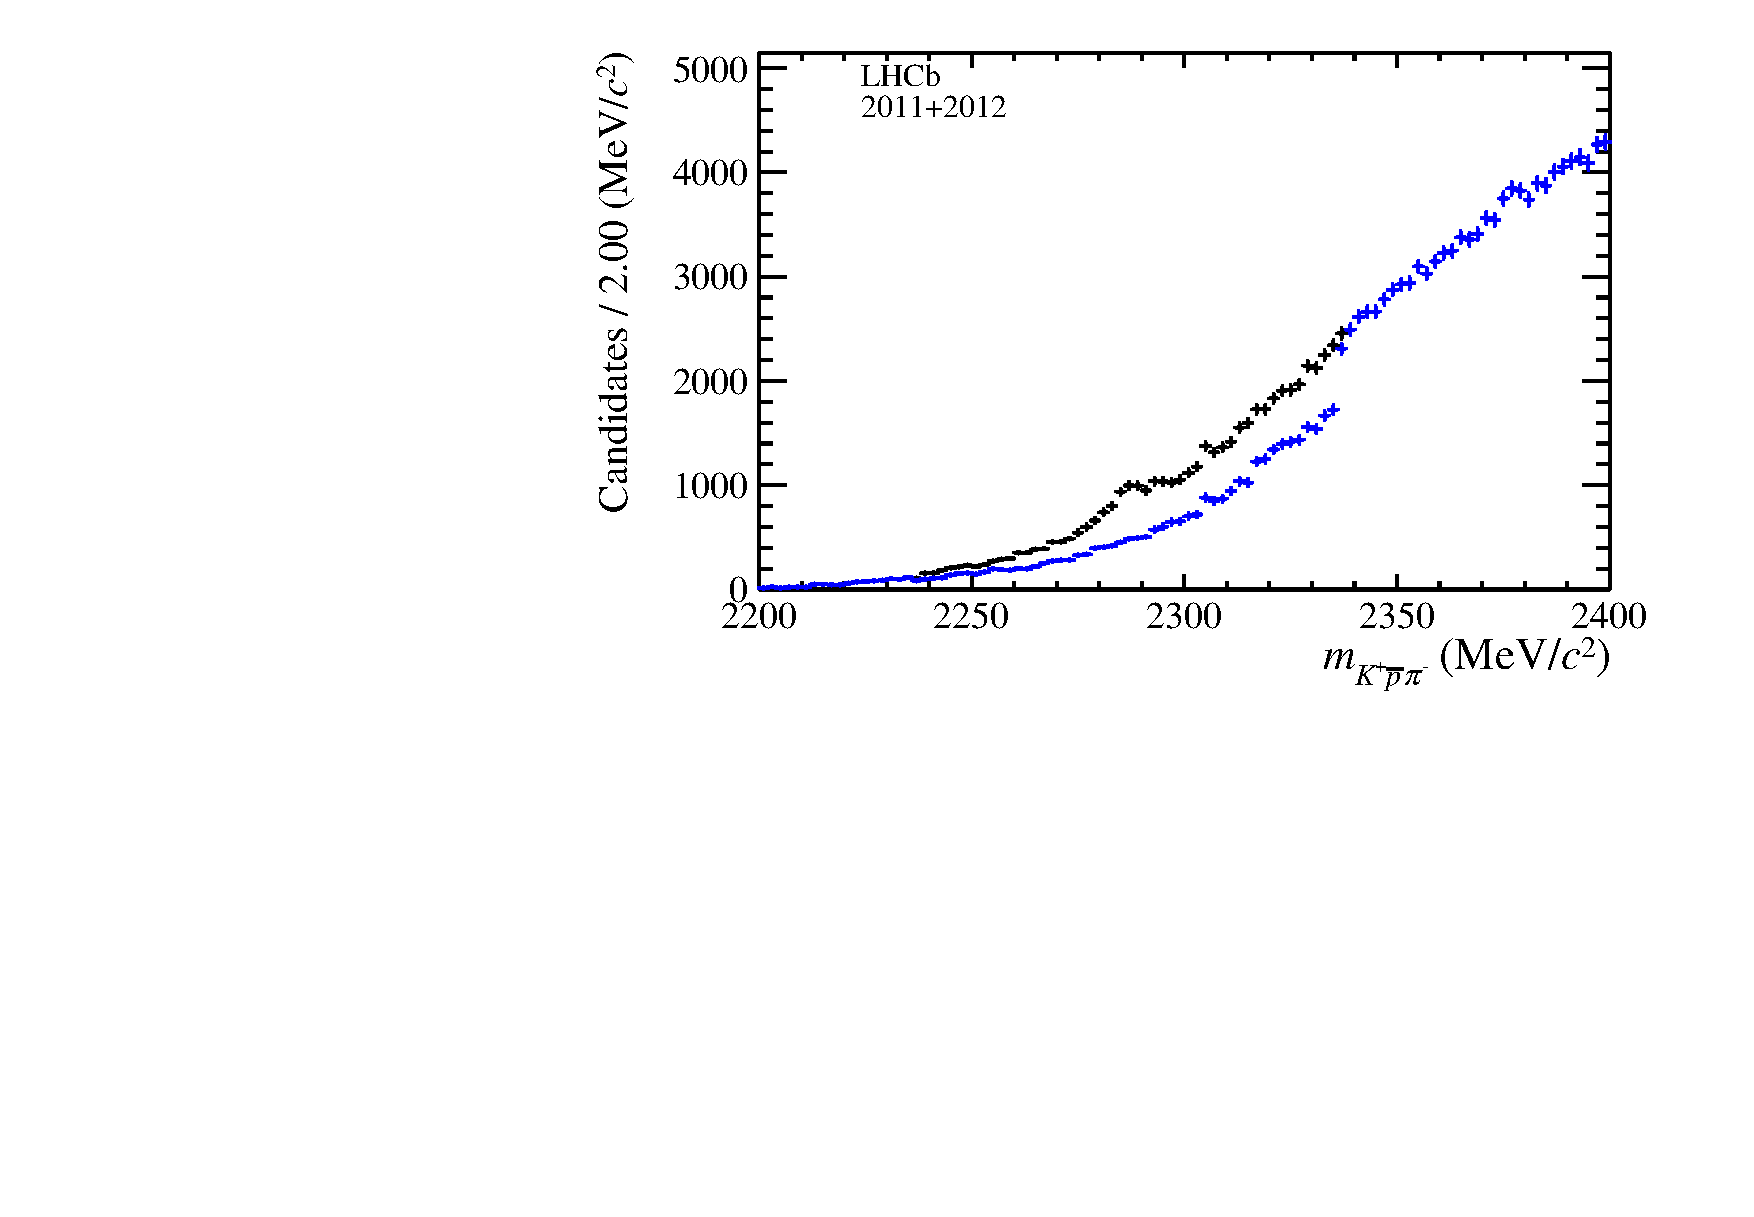
\includegraphics[width=0.49\textwidth]{06selection/figs/LcHypo1.pdf}
    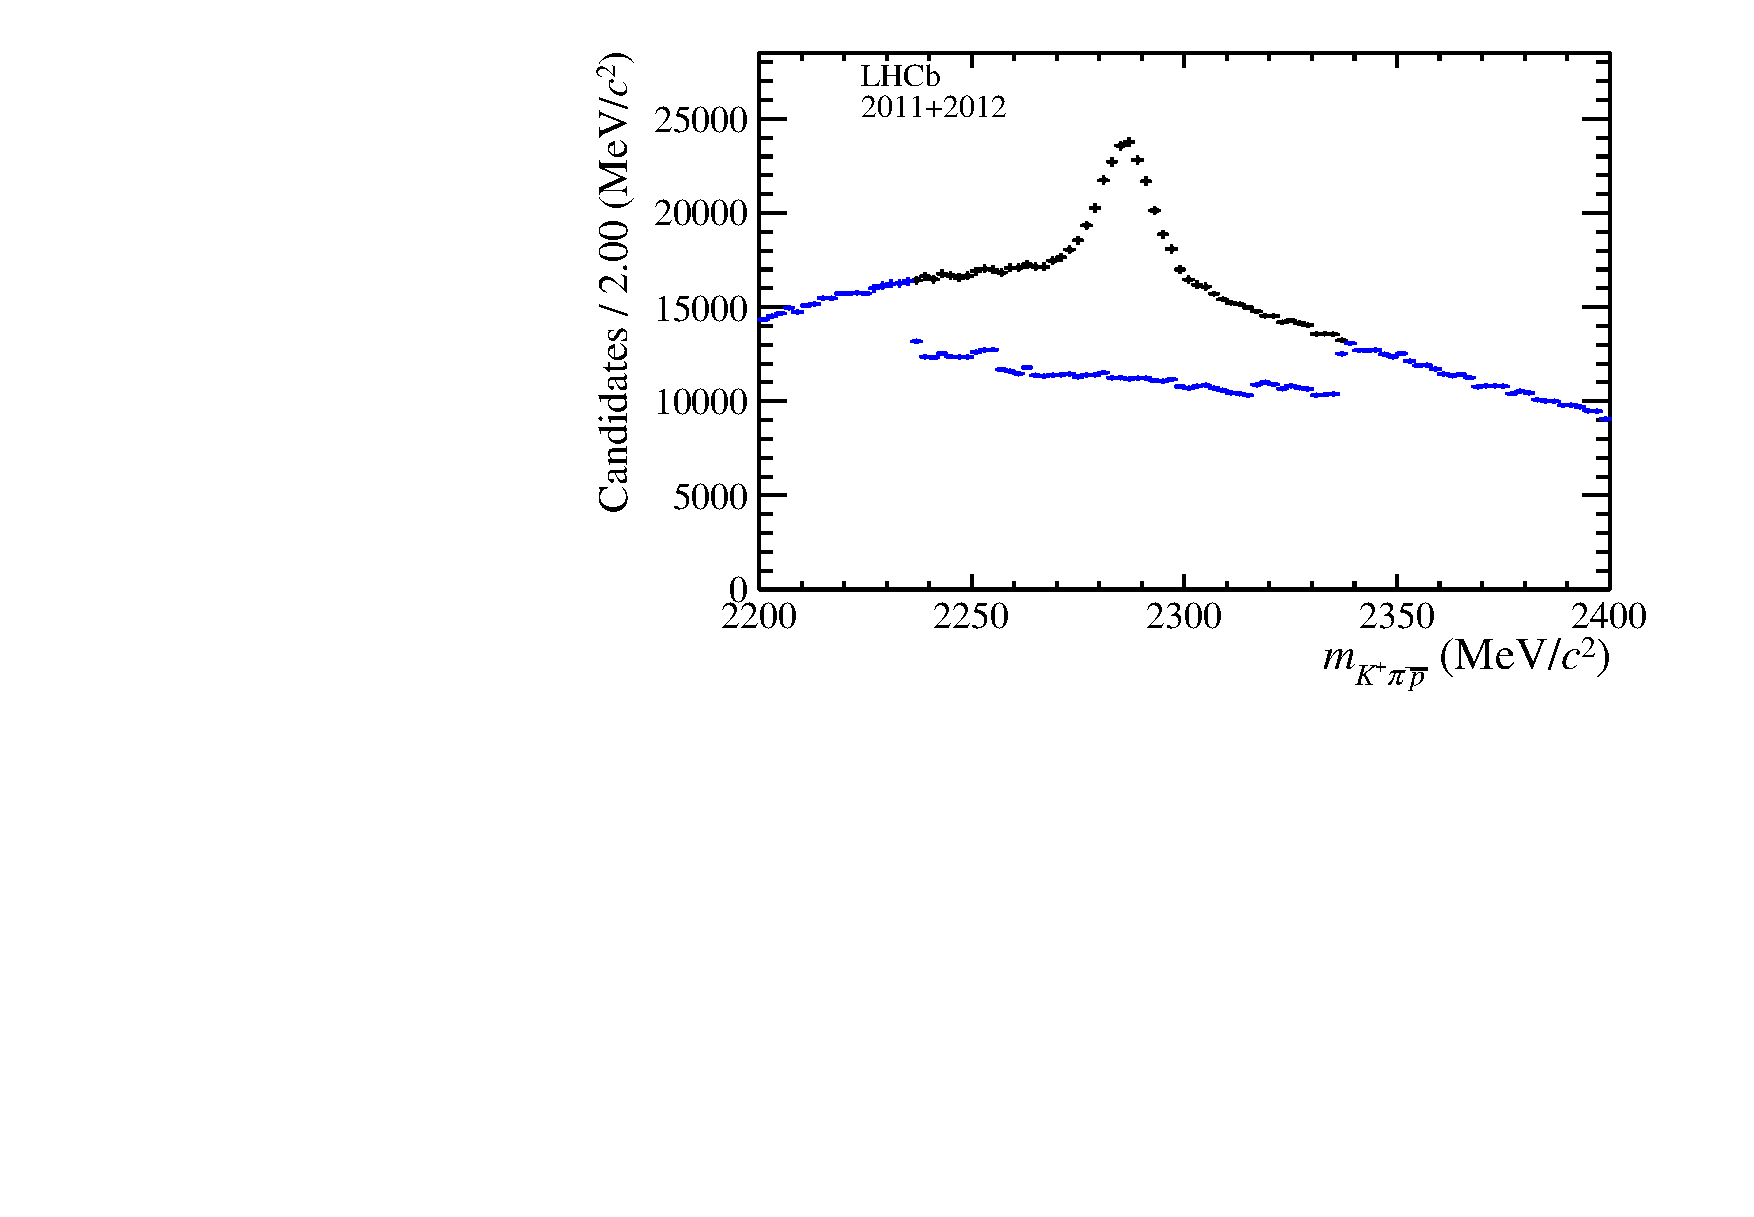
\includegraphics[width=0.49\textwidth]{06selection/figs/LcHypo2.pdf}
    \caption{Invariant mass distributions of the $\kaon\pion\proton$ combinations for both daughter pions of the \Dm-meson.
    The distributions are shown without the veto (black) and with the veto applied (blue).
    The left (right) plot shows the proton-mass hypothesis applied to the pion with lower (higher) transverse momentum.}
    \label{fig:LcVeto}
\end{figure}
To remove this background a two-stage veto is applied: In the first stage candidates are rejected if the invariant mass of the three hadrons is inside a \SI[per-mode=symbol]{30}{\MeVcc}  window around the nominal \Lcbar-mass $m_\Lcbar^{\text{PDG}}=\SI[per-mode=symbol]{2286.46}{\MeVcc}$ and the \dllppi is larger than \num{-8.0}.
In the second stage the mass window is enlarged to \SI[per-mode=symbol]{30}{\MeVcc} around the nominal \Lcbar-mass, but the \dllppi is loosened, only requiring $\dllppi>-5.0$.
After the preselection already \SI{99.720\pm0.004}{\percent} of the $\Lb\!\to\Lcbar\pip$ candidates are rejected.
This veto rejects another \SI{76.6\pm0.6}{\percent} at a signal efficiency of \SI{93.48\pm0.06}{\percent}.

In the same way as pions and protons can be misidentified it can happen that a kaon is falsely identified as one of the \Dm daughter pions.
Such misidentification gives rise to a potential background contamination from $\Bs\!\to\Dsm\pip$ candidates.
As before, for both pions a kaon mass hypothesis is applied and the three \Dm-daughters are combined.
However,  these distributions do not show a clear mass peak.
Therefore they are compared for different kinematic regions of the invariant $\left[\Kp\pim\pim\right]\pip$ mass: After applying the kaon mass hypothesis, $\Bs\!\to\Dsm\pip$ candidates should end up in the \Bs signal region, whereas no $\Bs\!\to\Dsm\pip$ candidates are expected in the upper-mass sideband $m_{\left[\Kp\pim\pim\right]\pip}>\SI[per-mode=symbol]{5500}{\MeVcc}$.
Therefore the invariant mass distributions of the \kaon\kaon\pion system are compared for candidates from the \Bs signal range \SIrange[per-mode=symbol]{5330}{5400}{\MeVcc} and a background range \SIrange[per-mode=symbol]{5500}{5700}{\MeVcc}.
The visible difference in \cref{fig:DsVeto} stems from the fact that those two distributions arise from different kinematic regions.
\begin{figure}[tbp]
    \centering
    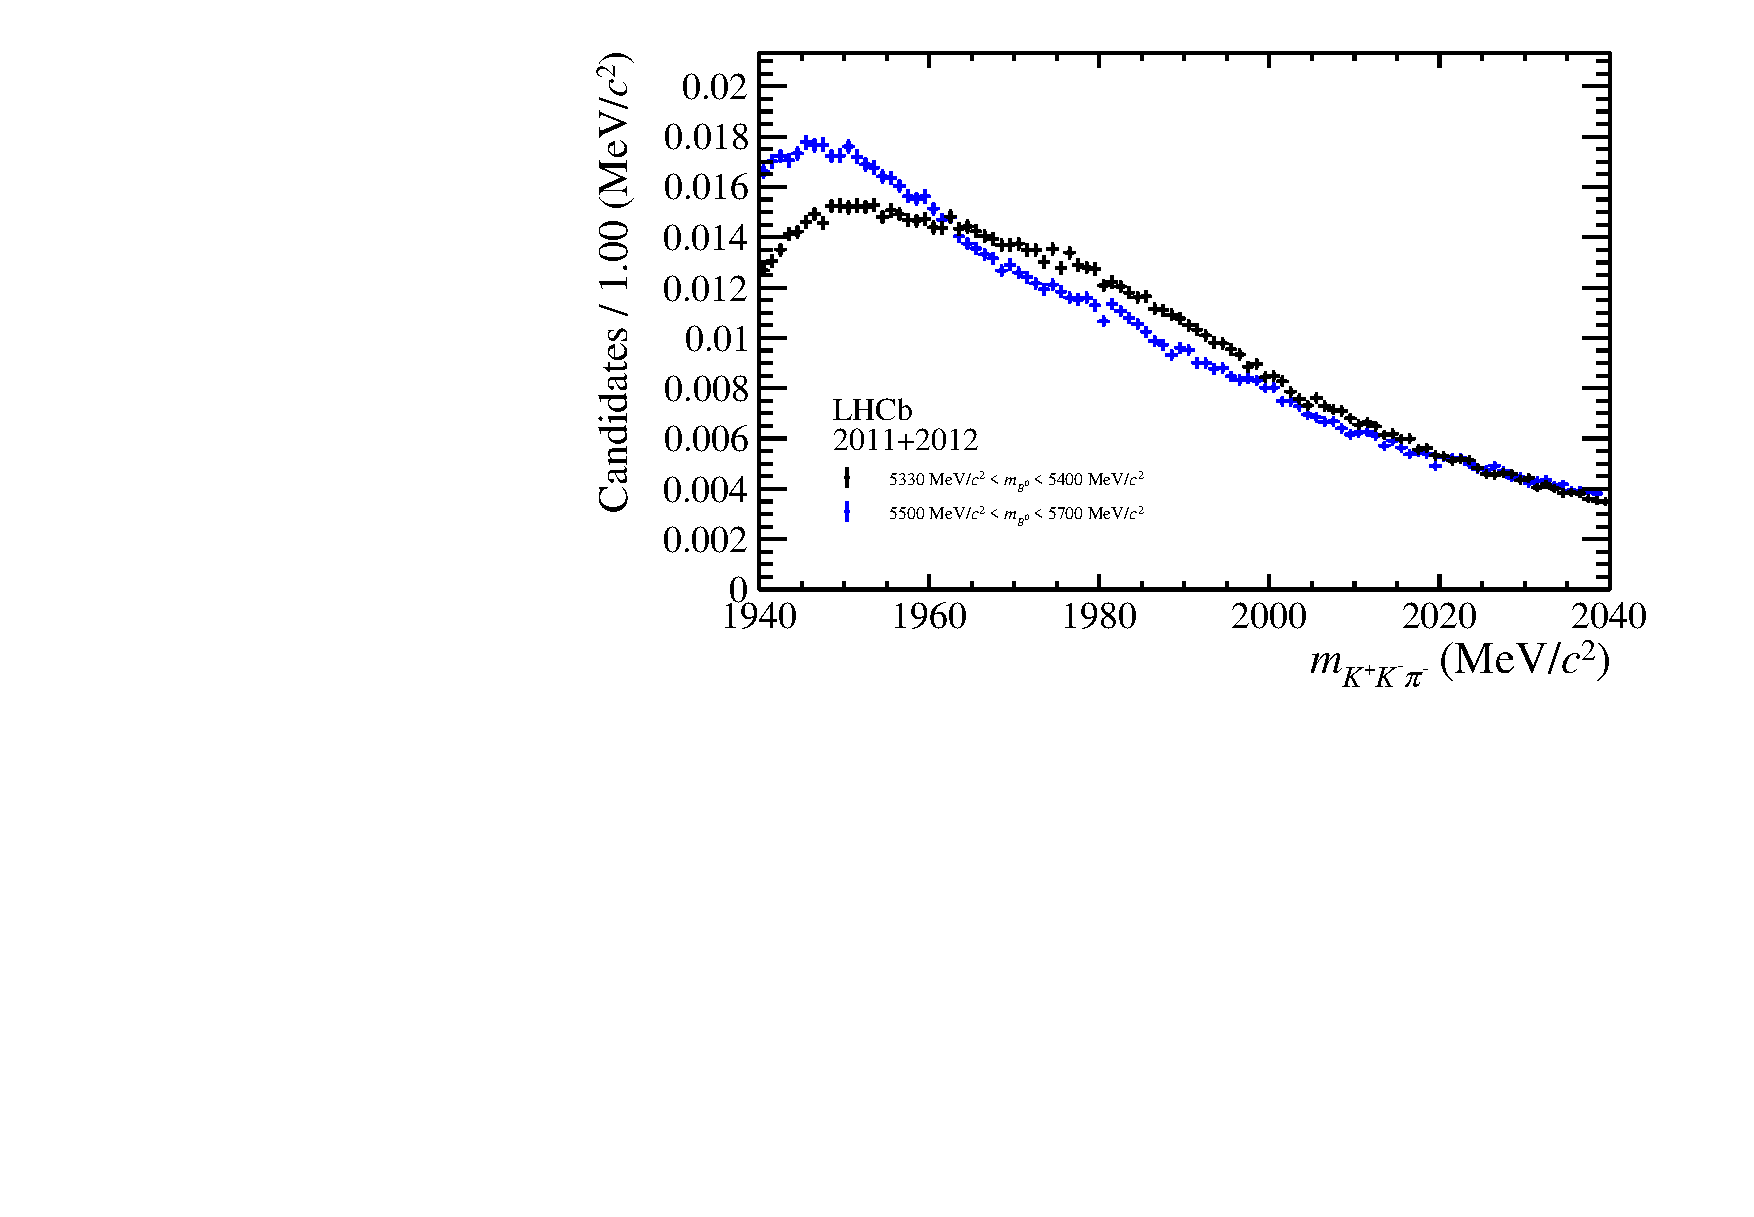
\includegraphics[width=0.49\textwidth]{06selection/figs/DsHypo1.pdf}
    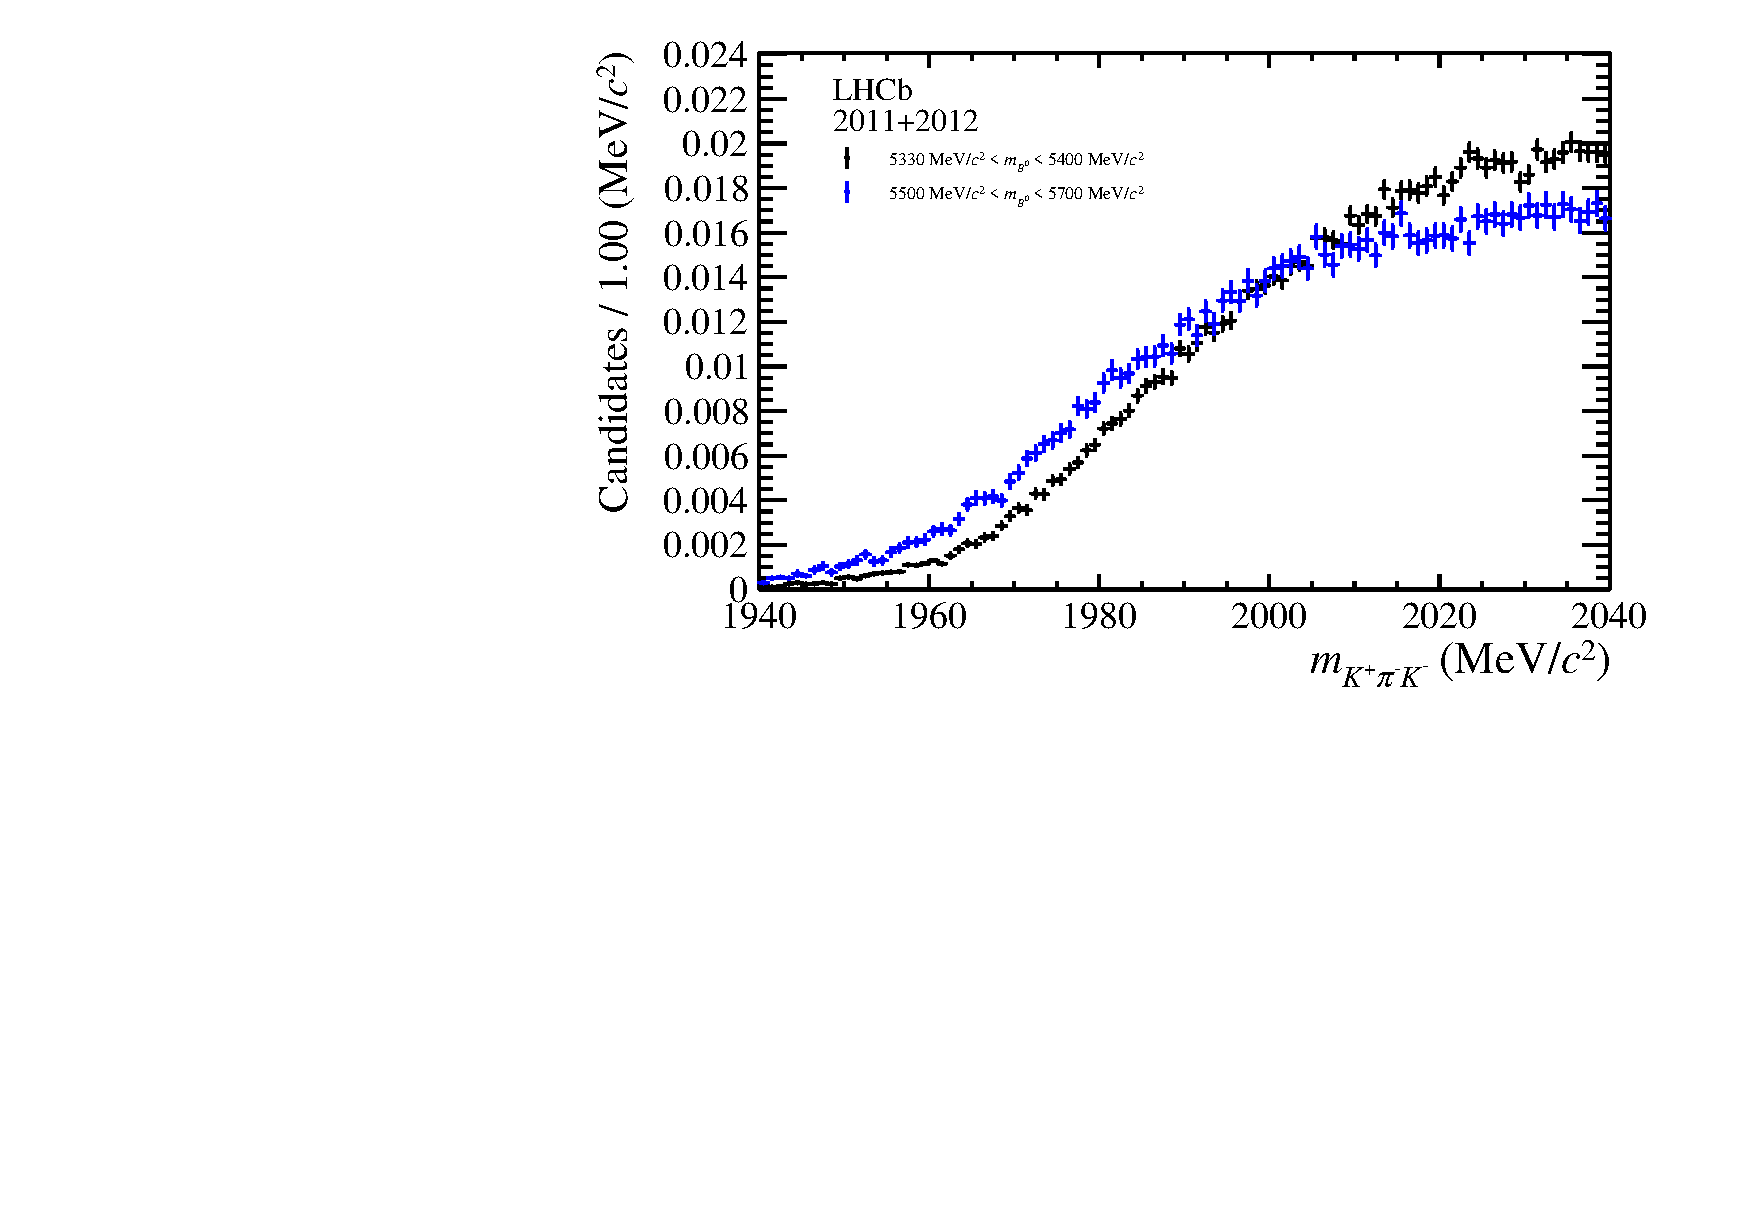
\includegraphics[width=0.49\textwidth]{06selection/figs/DsHypo2.pdf}
    \caption{Invariant mass distributions of the $\kaon\kaon\pion$ combinations for both daughter pions of the \Dm-meson.
    After applying the kaon mass hypothesis the distributions are shown in the \Bs signal region from \SIrange[per-mode=symbol]{5330}{5400}{\MeVcc} (black) and in a background region from \SIrange[per-mode=symbol]{5500}{5700}{\MeVcc} (blue).
    In the left plot the kaon-mass hypothesis is applied to the pion with lower transverse momentum, right to the pion with higher transverse momentum.}
    \label{fig:DsVeto}
\end{figure}
To further ensure that no significant contamination from $\Bs\!\to\Dsm\pip$ candidates is present in the data, resonances like \Kstarz- or $\phi$-mesons, which arise in possible \Dsm decays are studied.
Those resonances would become visible in the \kaon\kaon ($\phi$) and \kaon\pion (\Kstarz) invariant mass distributions.
Figure \ref{fig:phi_Kst_veto} shows exemplary the invariant mass distributions of the \kaon\kaon (\kaon\pion) combinations of the pion with larger transverse momentum under the kaon mass hypothesis with the daughter kaon (remaining daughter pion).
Additionally to the beforehand defined signal and background regions only candidates within a range from \SIrange[per-mode=symbol]{1940}{2040}{\MeVcc} from \cref{fig:DsVeto} are considered for these plots.
Consequently in the signal region a peaking structure would be expected in case of a significant contamination with $\Bs\!\to\Dsm\pip$ decays.
As no distribution in \cref{fig:DsVeto} and \cref{fig:phi_Kst_veto} shows such structure, background candidates from $\Bs\!\to\Dsm\pip$ decays are assumed to be negligible.
\begin{figure}[tbp]
    \centering
    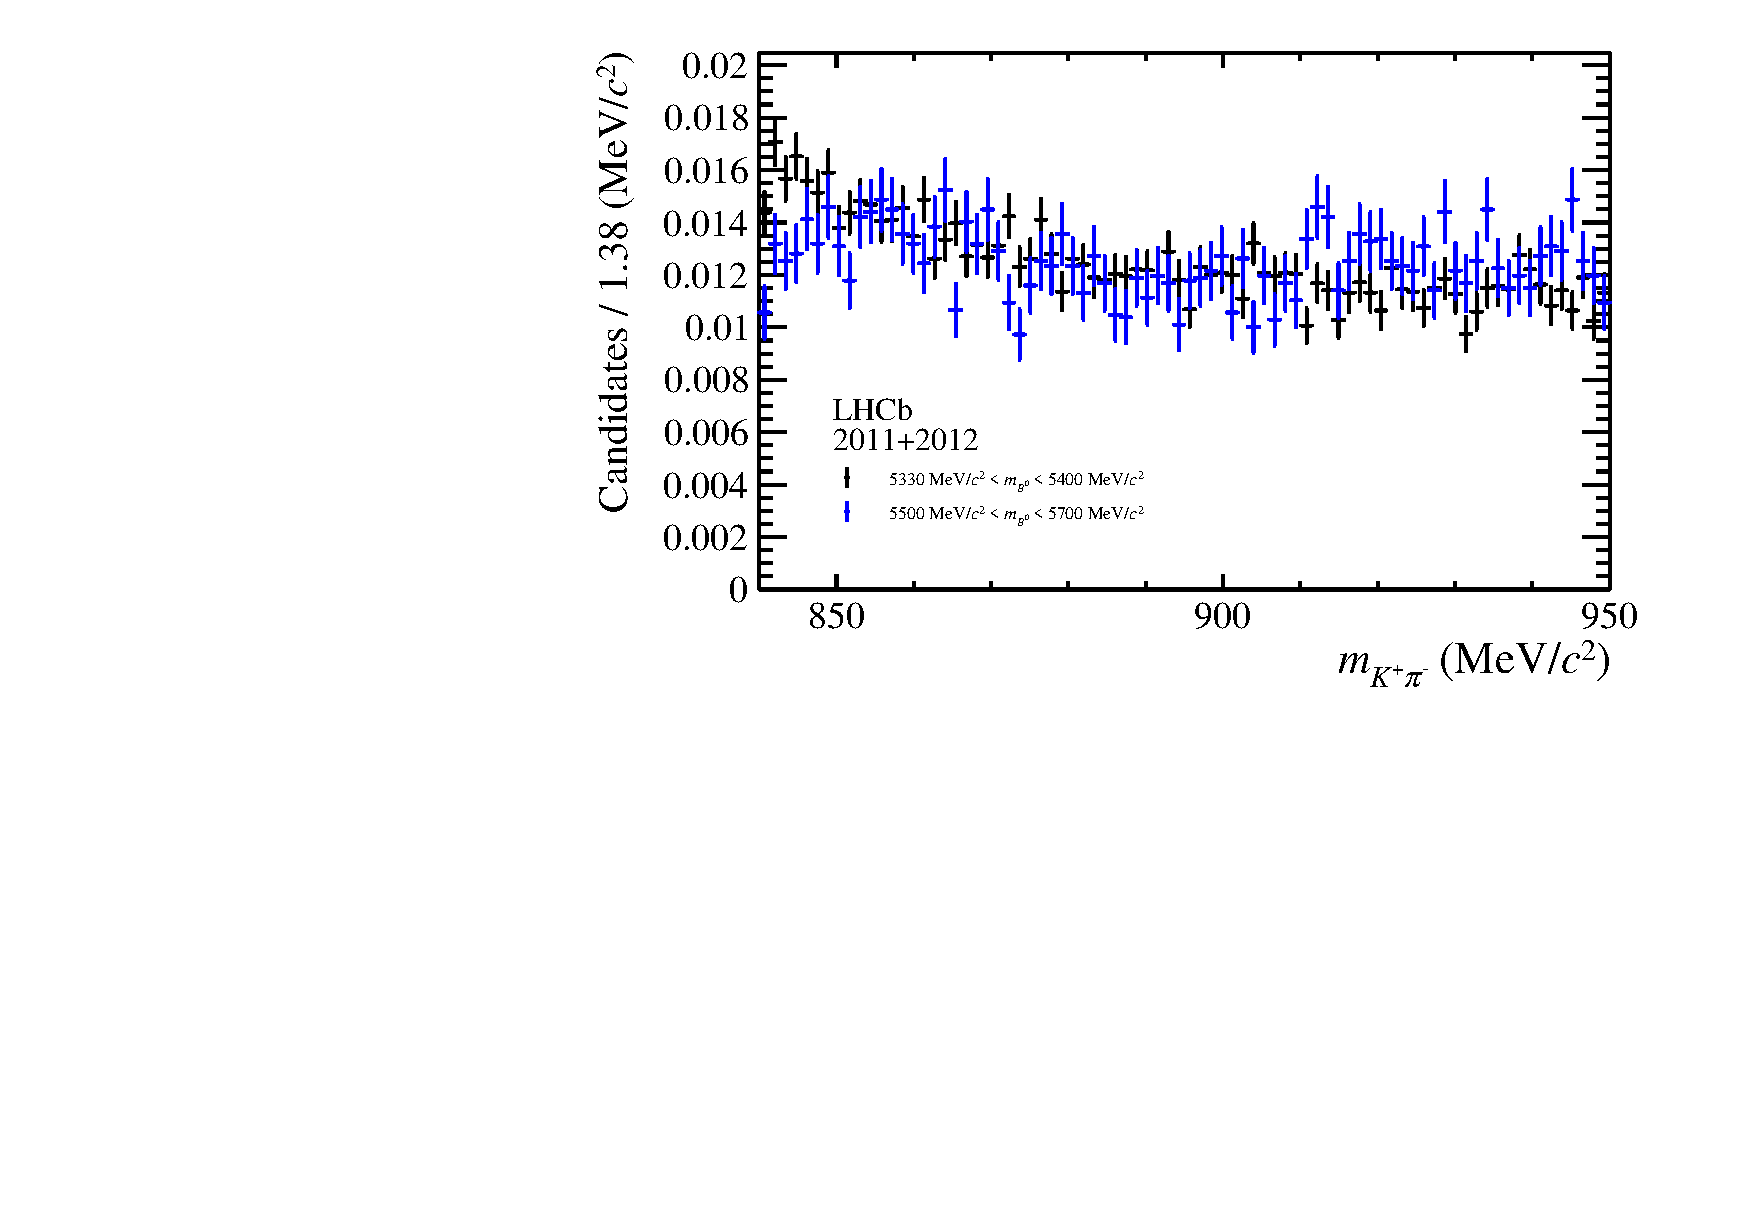
\includegraphics[width=0.49\textwidth]{06selection/figs/KstarHypo2.pdf}
    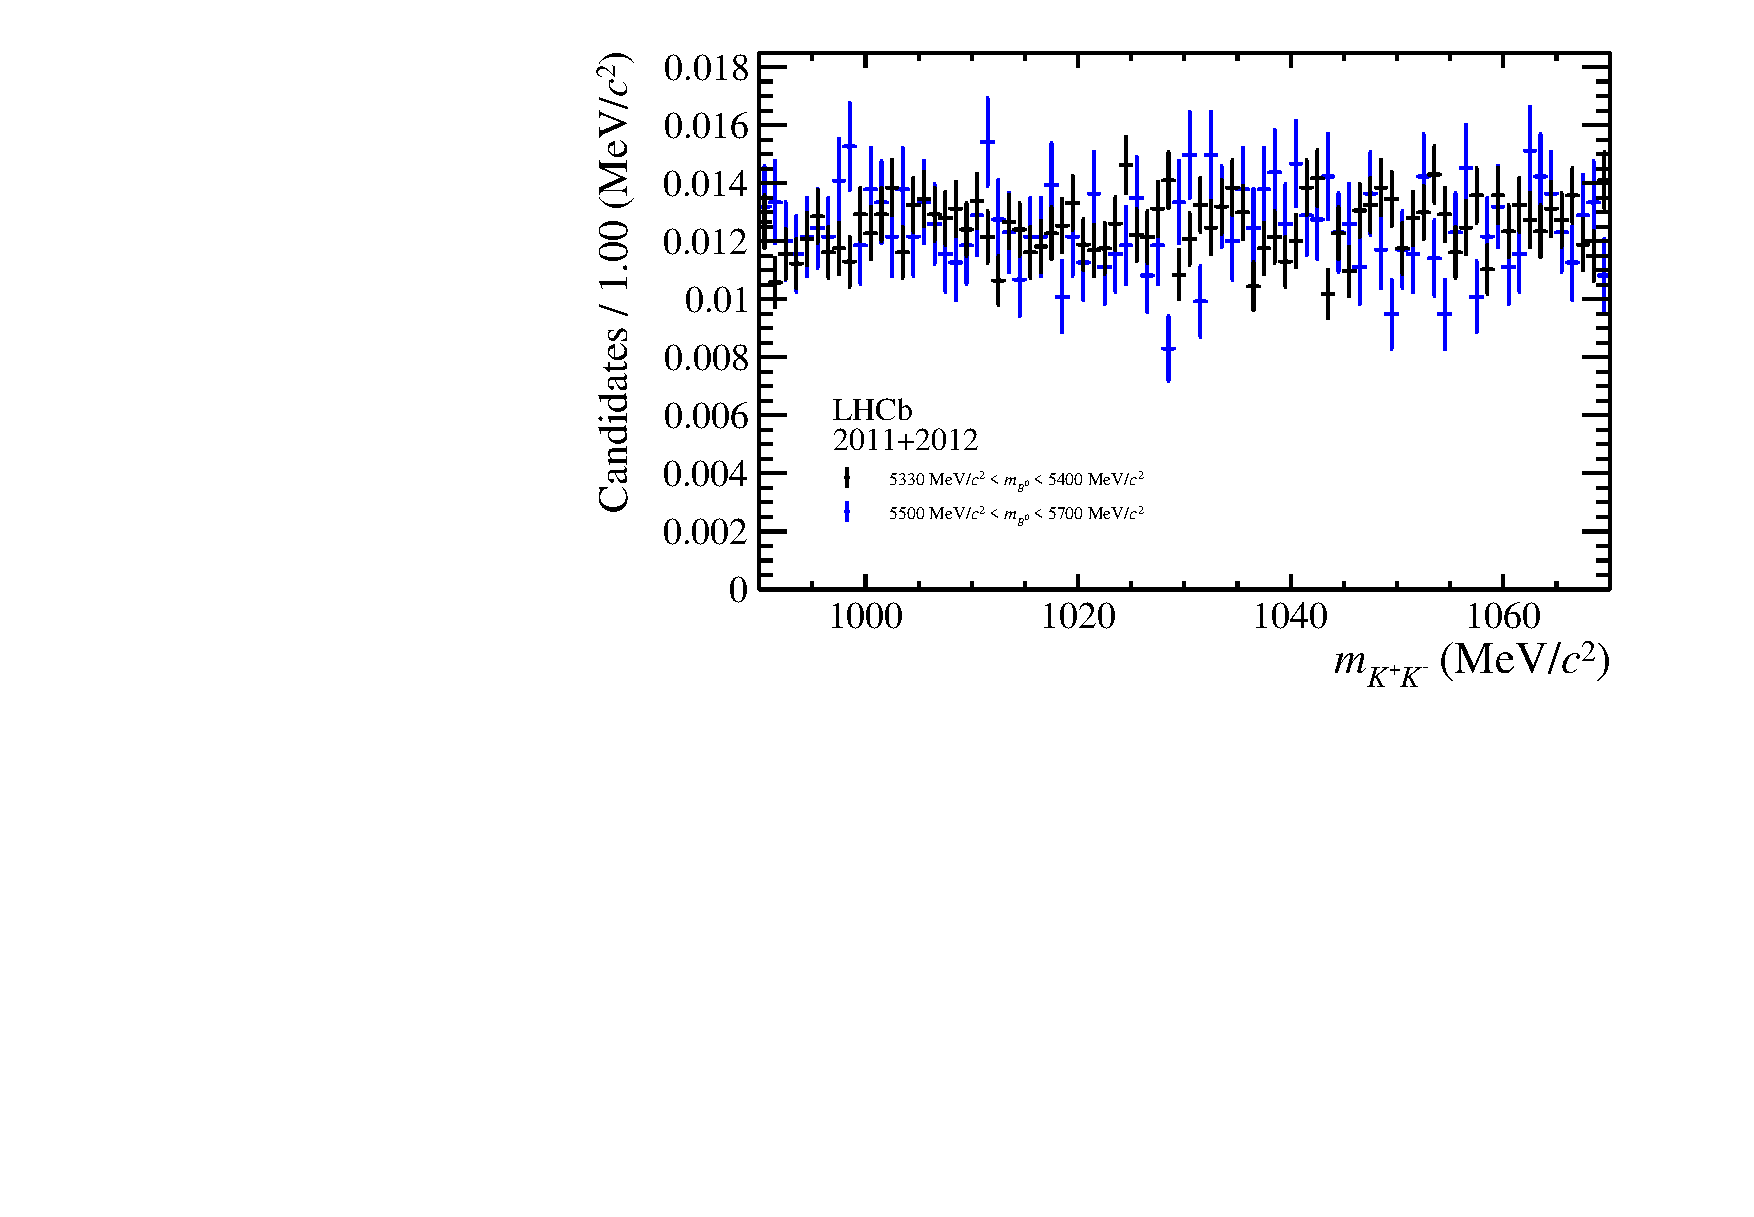
\includegraphics[width=0.49\textwidth]{06selection/figs/PhiHypo2.pdf}
    \caption{Invariant mass distributions of the \kaon\pion (left) and \kaon\kaon (right) combinations for the daughter pion of the \Dm-meson with larger transverse momentum with the daughter kaon or remaining daughter pion, respectively.
    Only candidates with $\SI[per-mode=symbol]{1940}{\MeVcc}<m_{\kaon\kaon\pion}<\SI[per-mode=symbol]{2040}{\MeVcc}$ are considered.
    The invariant mass distributions are shown in the in the \Bs signal region from \SIrange[per-mode=symbol]{5330}{5400}{\MeVcc} (black) and in a background region from \SIrange[per-mode=symbol]{5500}{5700}{\MeVcc} (blue).}
    \label{fig:phi_Kst_veto}
\end{figure}

The last background comes from $\Bz\!\to\DorDbar\kaon\pion$ decays, arising due to a kaon-pion misidentification of the bachelor track or a \Dm-daughter track, followed by a combination the bachelor track with a \Dm-daughter particle.
When doing the four possible combinations of applying the kaon hypothesis to the bachelor particle and the two \Dm-daughter pions all distributions show a flat shape.
Hence, backgrounds from $\Bz\!\to\DorDbar{}^0\kaon\pion$ decays are assumed to be negligible.
In \cref{fig:DzVeto} the combinations of the bachelor track with the \Dm-daughter pion with higher transverse momentum are shown for illustration.
\begin{figure}[tbp]
    \centering
    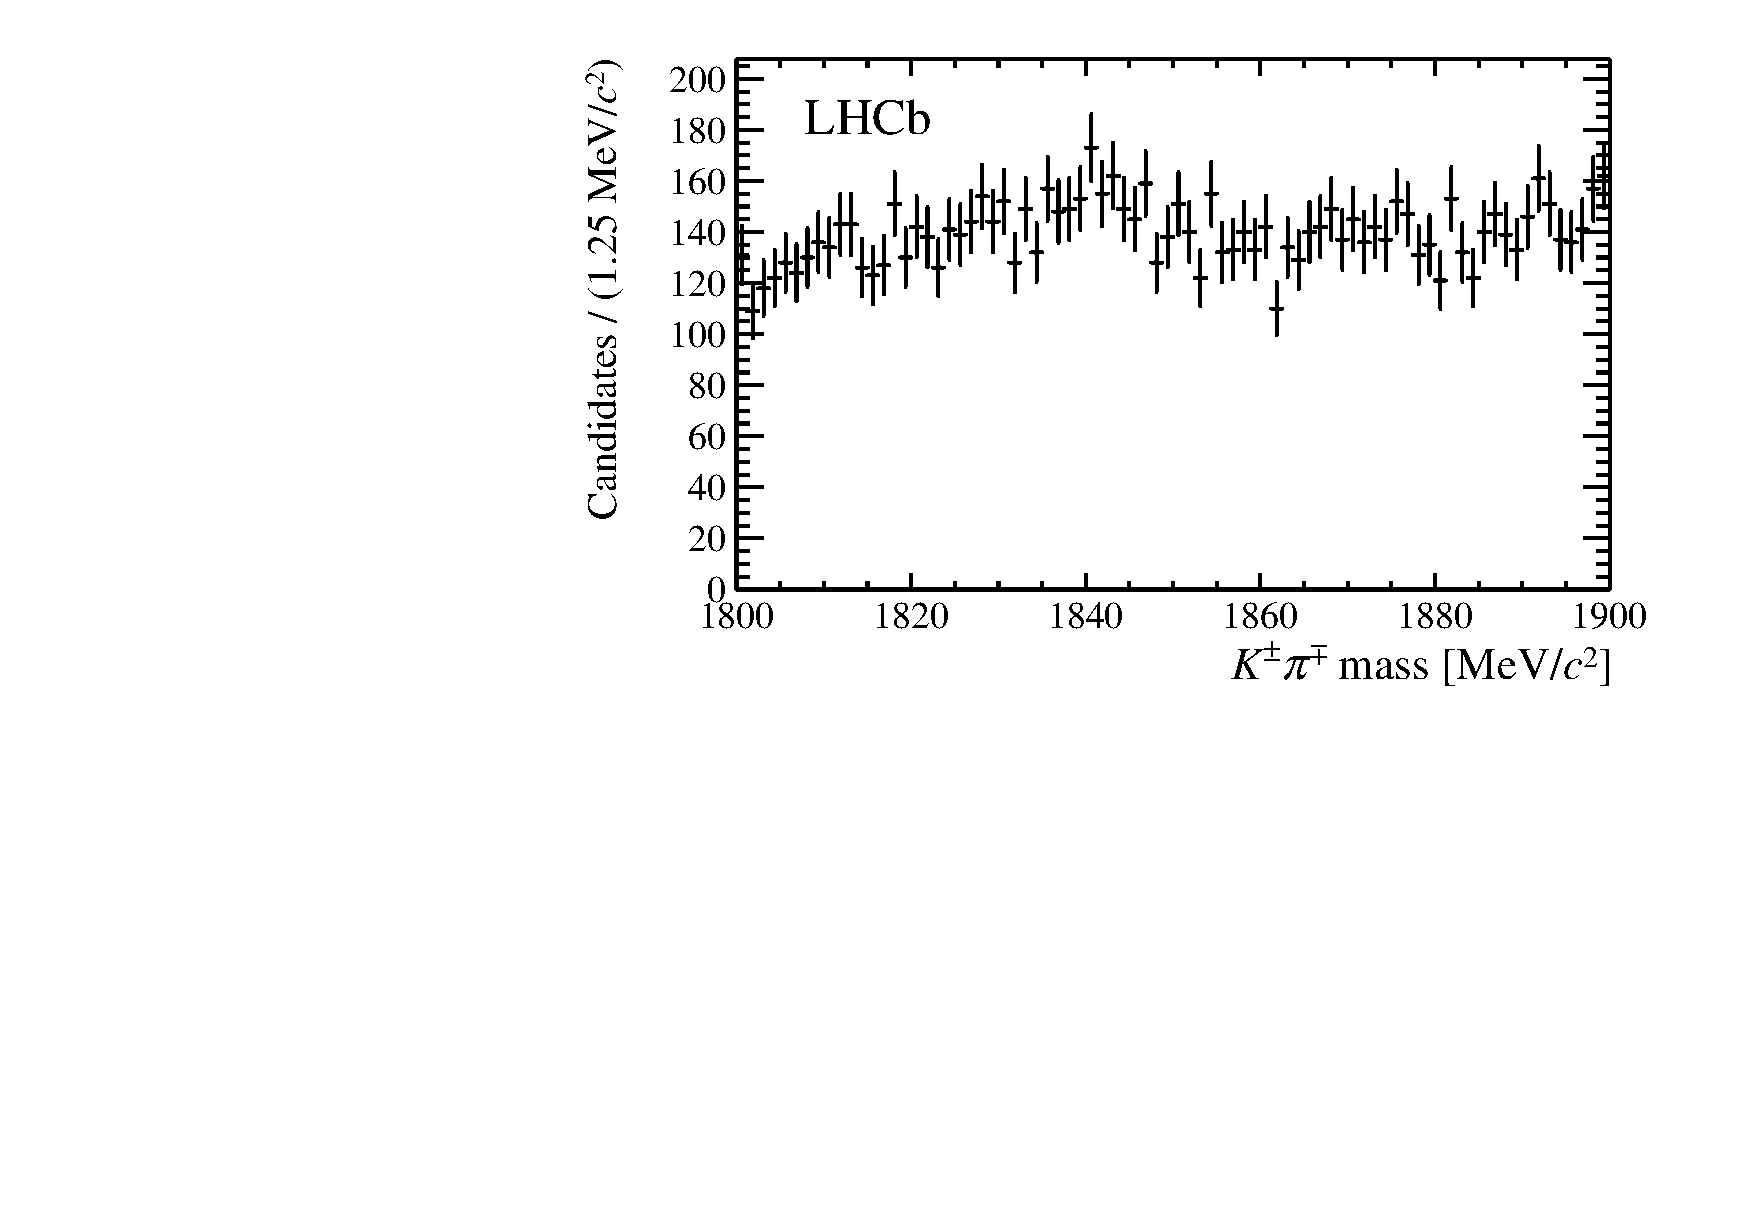
\includegraphics[width=0.49\textwidth]{06selection/figs/D0Hypo3.pdf}
    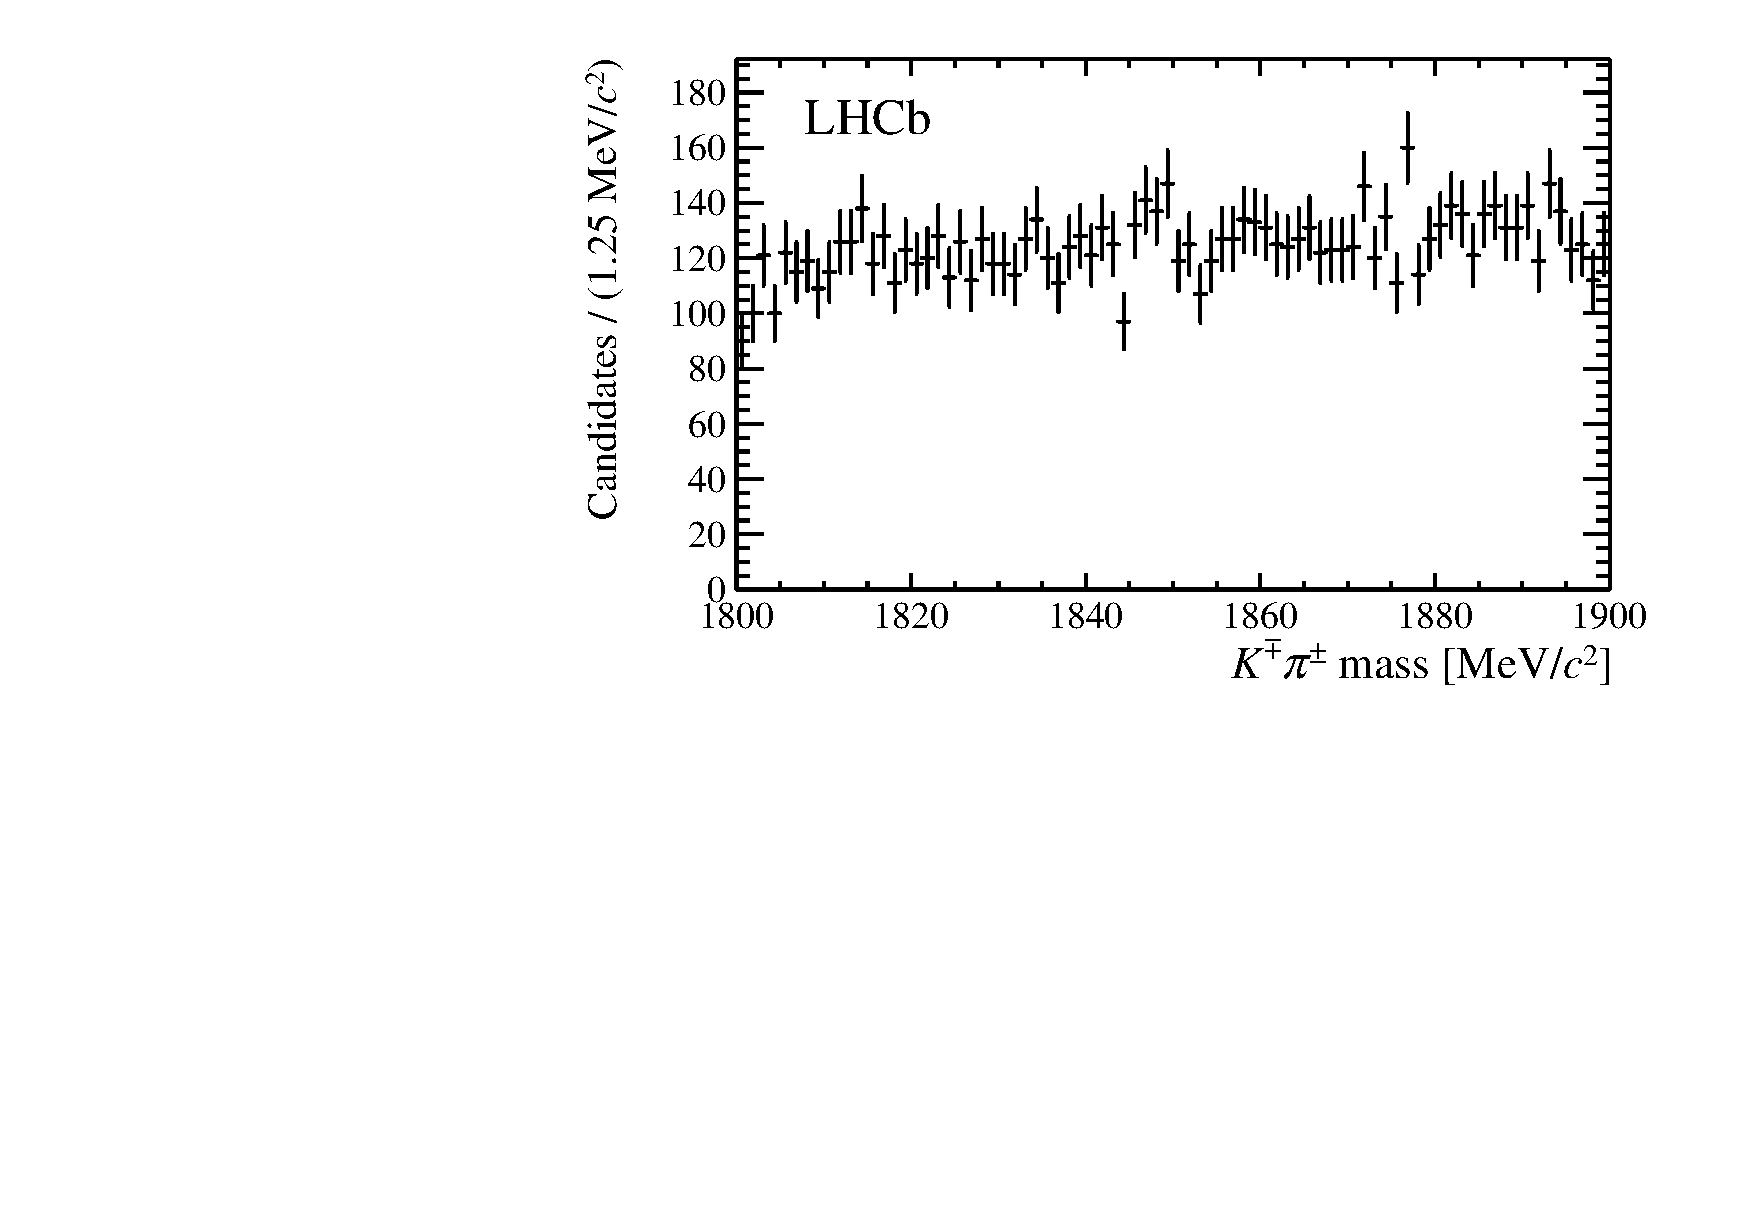
\includegraphics[width=0.49\textwidth]{06selection/figs/D0Hypo4.pdf}
    \caption{Invariant mass distributions for the combinations of the bachelor particle with the \Dm-daughter pion with higher transverse momentum.
    In the left plot the kaon hypothesis is applied to the bachelor pion, the right plot shows the kaon hypothesis applied to the \Dm-daughter pion.}
    \label{fig:DzVeto}
\end{figure}

\subsubsection*{Wrongly associated PVs}

The average number of \proton\proton-collisions per bunch crossing is $\nu=2.5$.
Therefore a considerable amount of events has more than one \ac{PV} and in these events a \Bz candidate can be associated with each of them.
Besides that an event can also contain more than one \Bz candidate; in this case the \Bz candidate is chosen randomly (more details in \cref{sec:MultCands}).
However, in case of multiple \ac{PV}s per event the \Bz candidate can be associated with the wrong PV what leads to a wrong decay time for this candidate.
Usually a decay time dependent selection efficiency is expected at \lhcb, which strongly increases at small decay times up to $\approx\SI{2}{\pico\second}$ and shows a flat or slightly dropping distribution for high decay times.
This efficiency, further denoted as decay time acceptance, is caused by the track reconstruction in the \velo and certain trigger requirements (more details are given in \cref{sec:acceptance}).
Yet, due to the wrong \ac{PV} association a large, unexpected tail at high decay times arises.
This can be checked on simulation, where the true decay time is known.
Weighting each (\Bz,\ac{PV})-candidate with an exponential using the true lifetime of the \Bz candidates - \ie (\Bz,\ac{PV})-candidates with high decay times get higher weights - shows an excess of (\Bz,\ac{PV})-candidates at high decay times (see \cref{fig:WrongPVMC}).
\begin{figure}[tbp]
    \centering
    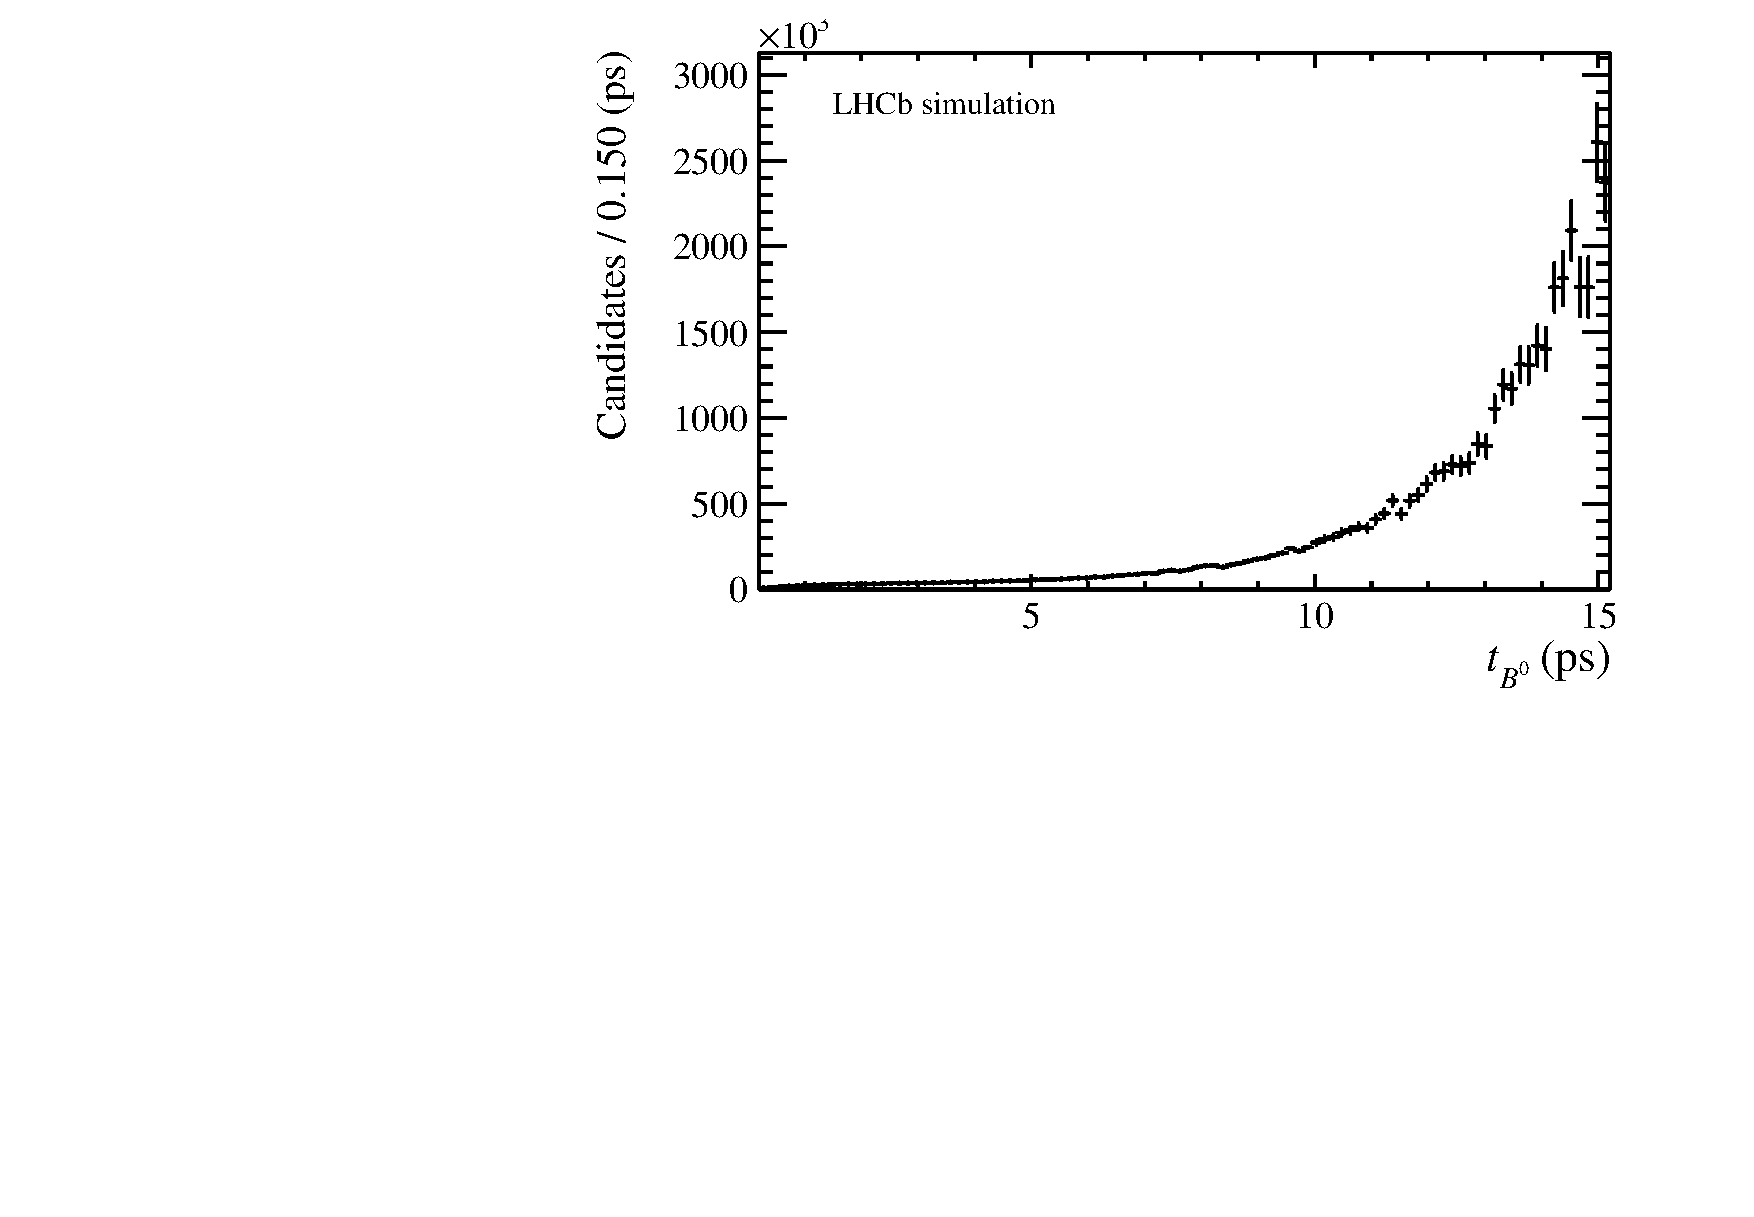
\includegraphics[width=0.45\textwidth]{06selection/figs/WrongPVs-weightedBad.pdf}
    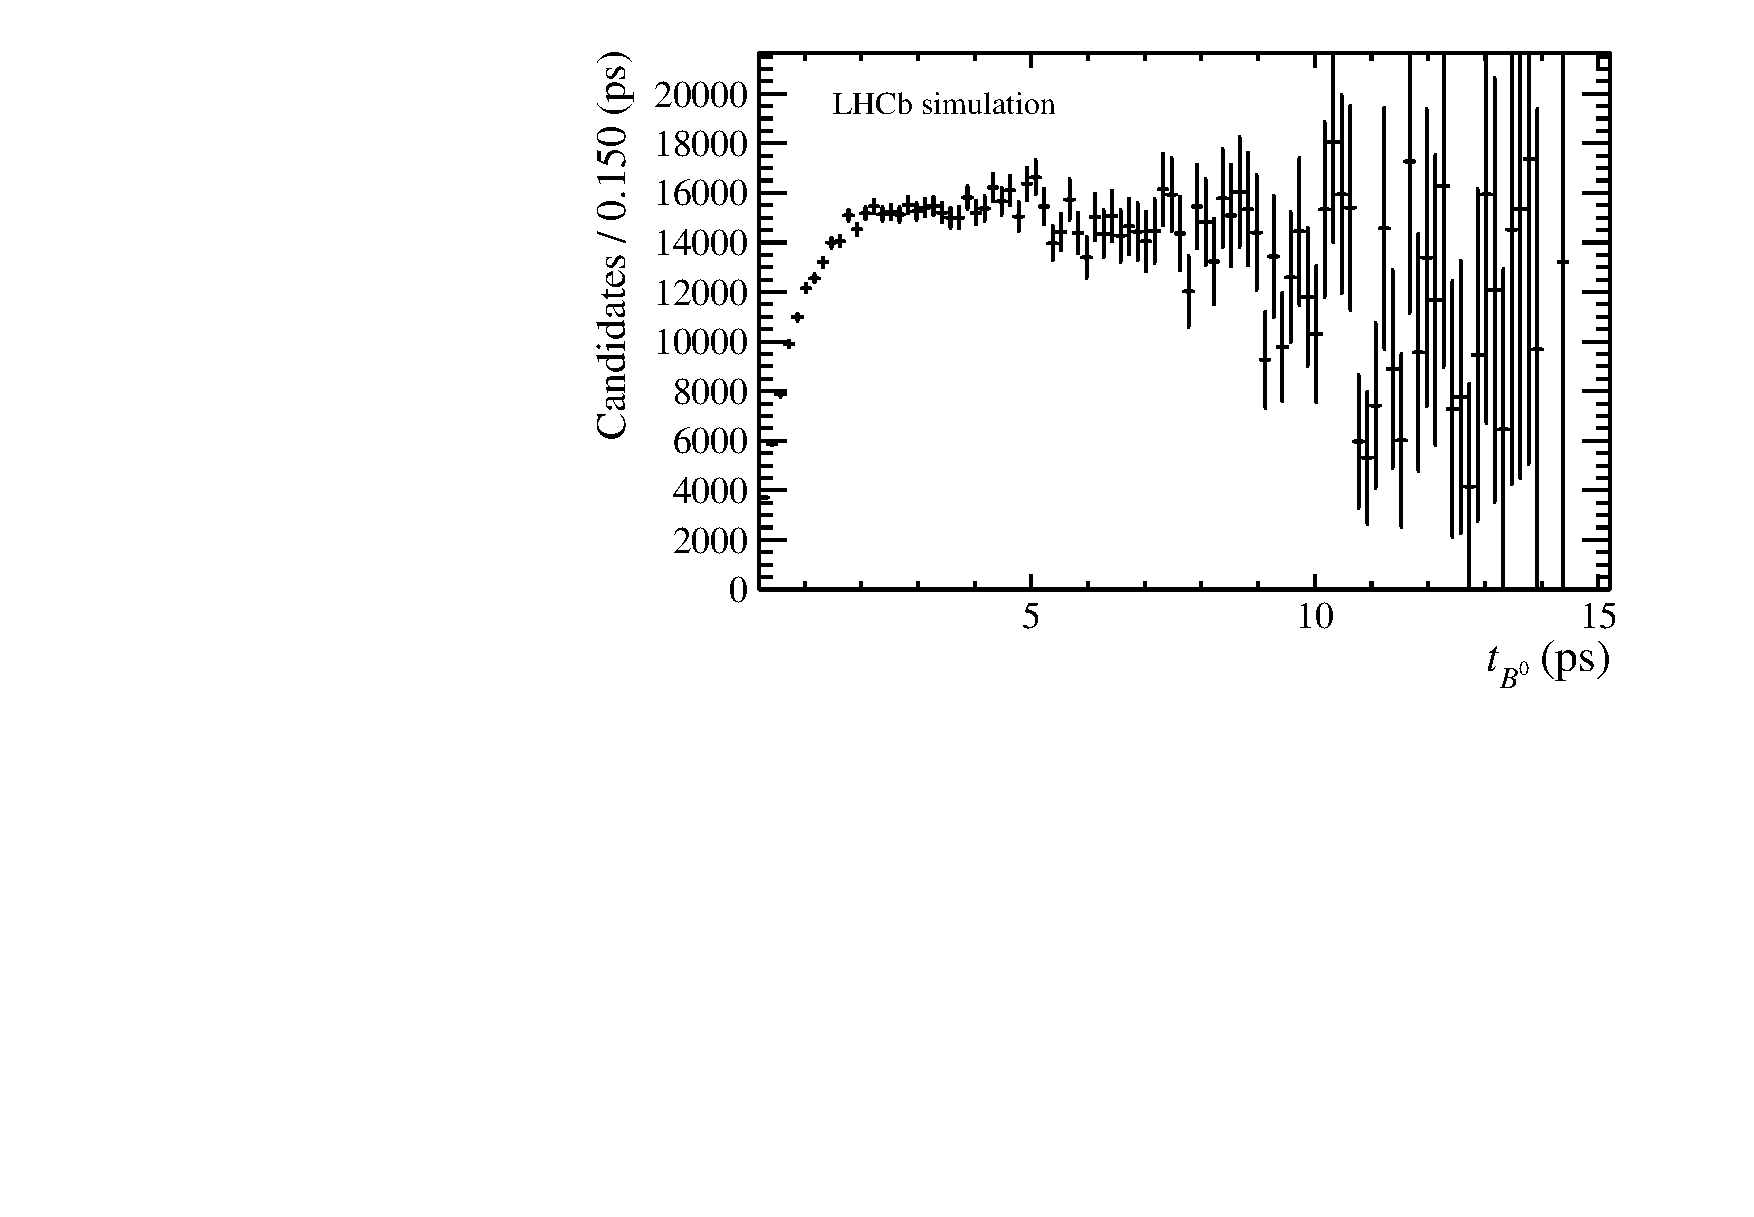
\includegraphics[width=0.45\textwidth]{06selection/figs/WrongPVs-weightedGoodMC.pdf}
    \caption{Left: Decay time distribution of simulated \BdToDpi candidates, wheighted with an exponential using the true lifetime of the \Bz candidates.
    At high decay times an excess of (\Bz,\ac{PV})-candidates can be seen.
    Right: Decay time distribution of simulated \BdToDpi candidates, wheighted with an exponential using the true lifetime of the \Bz candidates after applying a cut on the distance between the true and the reconstructed $z$ position of the \ac{PV}.
    The expected acceptance distribution at \lhcb is visible.}
    \label{fig:WrongPVMC}
\end{figure}
Further on simulation the true $z$-position of the \ac{PV} is known and can be compared with the reconstructed $z$-position.
Requiring that the distance between the true $z$-position of the \ac{PV} and the reconstructed $z$-position does not exceed five times the uncertainty on the reconstructed $z$-position removes the wrong associated (\Bz,\ac{PV})-candidates from the sample and the expected decay time acceptance becomes visible (\cref{fig:WrongPVMC}).
Though, this approach cannot be applied to data.
Therefore a criterion is developed requiring for each (\Bz,\ac{PV})-candidate the impact parameter $\chi^2_{\text{DTF,PV}}$ with any other \ac{PV} in the event ($\text{MinIP}\chi^2$) to be larger than a certain value.
This means that in case this $\text{MinIP}\chi^2$ is too small, the two corresponding \ac{PV}s cannot be distinguished sufficiently well from each other, and the (\Bz,\ac{PV})-candidate is rejected.
Events which contain just one \ac{PV} are kept always.
The cut is optimised in such a way, that \SI{98}{\percent} of the events in the simulated \BdToDpi sample are retained.
In \cref{fig:WrongPVData} the distribution of the $\text{MinIP}\chi^2$ variable together with the cut point at \num{16.5} and the resulting decay-time-acceptance distribution after applying the \enquote{data} criterion on simulation is shown.
\begin{figure}[tbp]
    \centering
    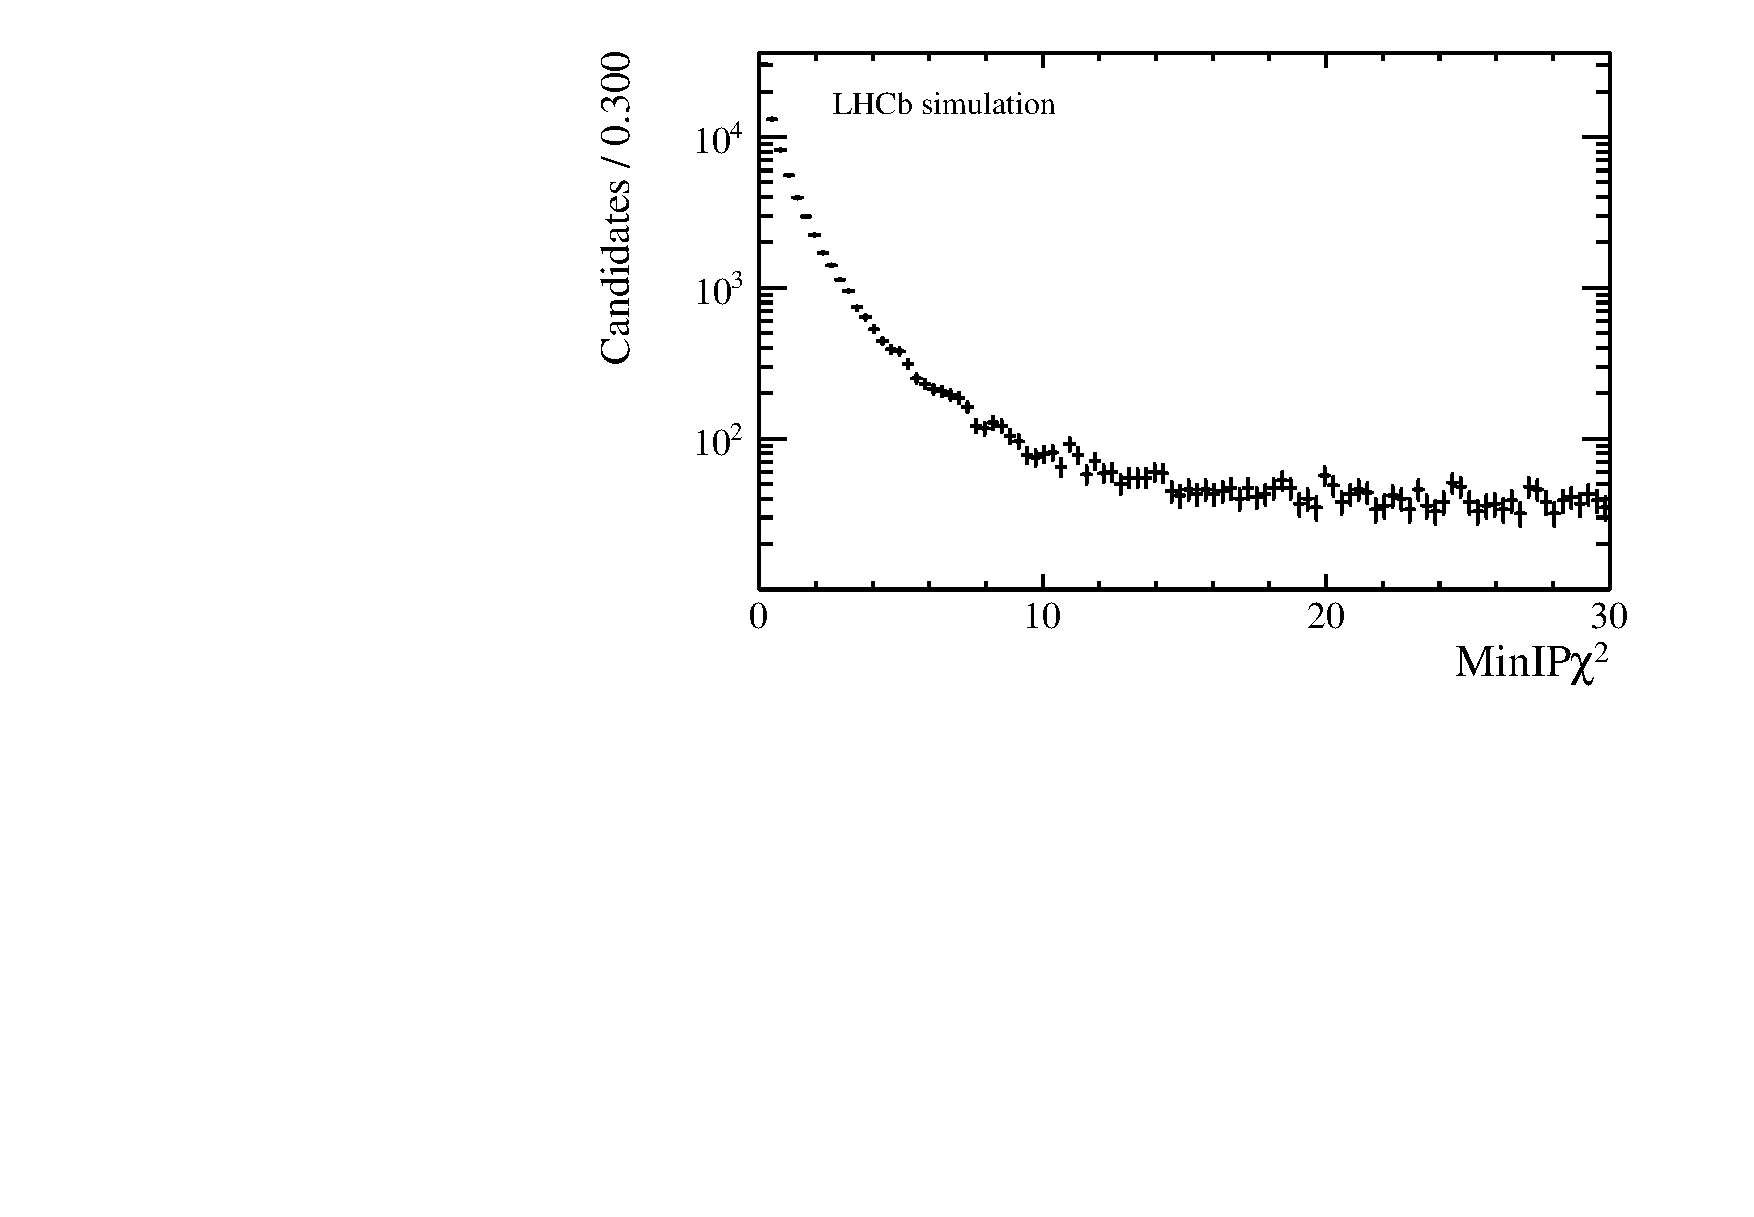
\includegraphics[width=0.45\textwidth]{06selection/figs/MinIPCHI2.pdf}
    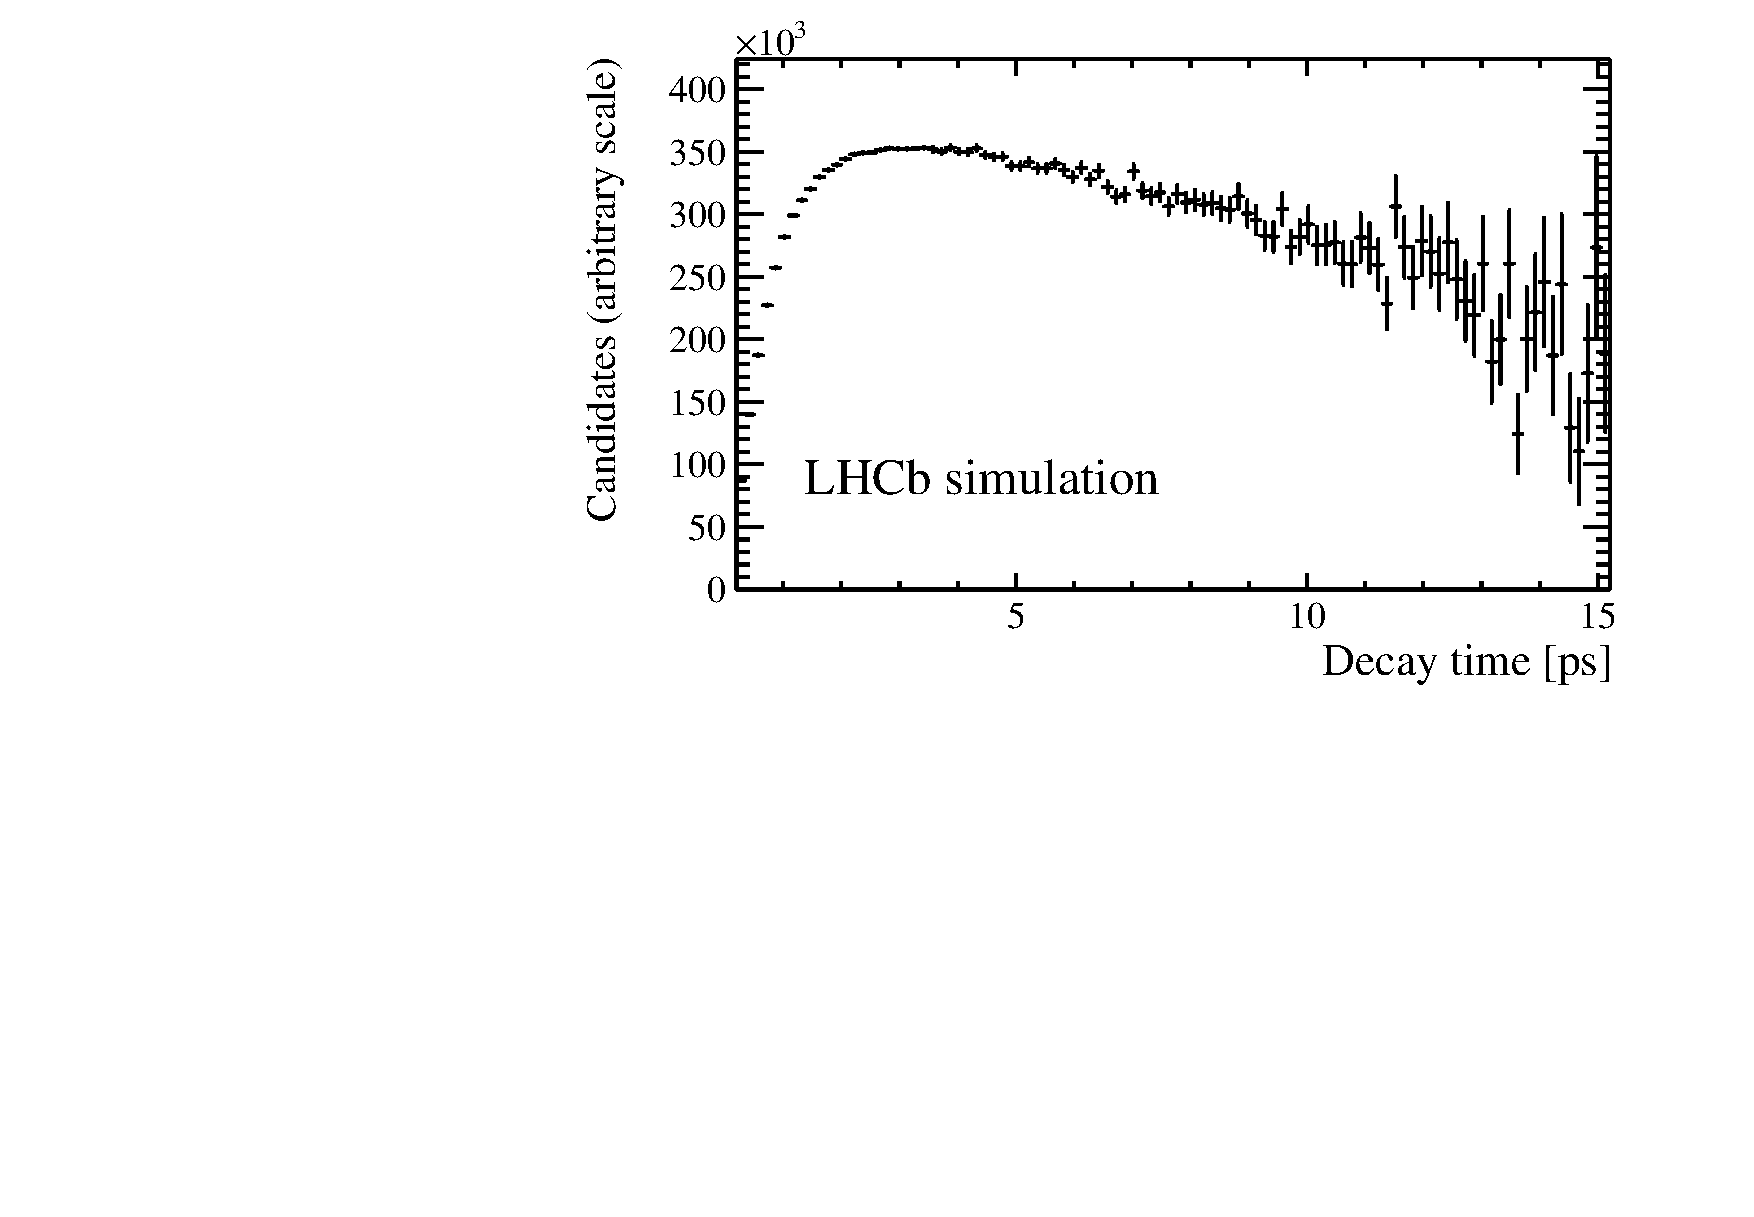
\includegraphics[width=0.45\textwidth]{06selection/figs/WrongPVs-WeightingGoodData.pdf}
    \caption{Left: Distribution of the $\text{MinIP}\chi^2$ variable with the chosen cut point in a narrow range.
    For larger values of $\text{MinIP}\chi^2$ the distribution remains flat.
    Candidates with $\text{MinIP}\chi^2<=16.5$ are rejected.
    Right: Decay time distribution of simulated \BdToDpi candidates, wheighted with an exponential using the true lifetime of the \Bz candidates after applying the cut on $\text{MinIP}\chi^2$.
    The expected acceptance distribution at \lhcb is visible.}
    \label{fig:WrongPVData}
\end{figure}

In contrast the \ac{PV} could also be chosen using some \enquote{best} \ac{PV} criterion, \eg picking the \ac{PV} with the smallest $\text{IP}\chi^2$ w.r.t the \Bz candidate.
Such criterion also removes most of the wrongly associated \ac{PV}s, but potentially biases the decay time distribution, whereas the strategy described above treats all \ac{PV}s equally and thus the decay time distribution remains unbiased.

\subsection{Development of a MVA classifier}
\label{sec:MVADev}

Combinatoric background is suppressed using a \ac{MVA}, more precisely a \ac{BDT} is used.
A \ac{BDT} is a machine learning algorithm for classification.
As all machine learning algorithms it needs to learn, which classes of events should be separated.
Therefore it needs training samples, consisting only of events of the respective classes.
In this case \BdToDpi candidates should be separated from combinatorial background candidates and therefore it needs to be provided with proxies for these classes of candidates.
As proxy for the \BdToDpi candidates, simulation is used based on the conditions of the \num{2012} data taking.
The upper-mass sideband of the \num{2012} data with $m_{\left[\Km\pip\pip\right]\pim}>\SI[per-mode=symbol]{5500}{\MeVcc}$ mimics the background.
Further both proxy samples are divided into a training and a test sample of same size.
When training the \ac{BDT}, the training part is used to actually classify the candidates, while the \ac{BDT} can be applied on the independent test sample to check whether the performance is the same on both samples.
If the performance is different, the \ac{BDT} shows so-called overtraining, \ie the classifier is optimised on statistical fluctuations of the training samples and cannot be applied to other independent samples without a loss in performance.
Another powerful test to check for overtraining is to compare the output distribution of the \ac{BDT} between the training and test sample - again, a difference would indicate that the \ac{BDT} is overtrained.
Since the \ac{BDT} should also in this case learn to separate signal candidates from combinatoric background after applying the vetoes and removing backgrounds like $\Lb\!\to\Lcbar\pip$, all previous selection steps are applied to the signal- and background-proxy samples.

In total, the \ac{BDT} uses \num{16} input variables which are listed in \cref{tab:BDTInput}.
To reduce the number of input variables, from pairs of variables which have a correlation of \SI{97}{\percent} or larger the variable with the smaller separation power is removed.
The final variables cover mostly various $\text{IP}\chi^2$ variables, flight distances, momenta and flight directions.
Furthermore, the $\chi^2$ of the DTF with a constraint on the \ac{PV} is added, as it shows a good separation power between \BdToDpi signal candidates and combinatoric background candidates.
\begin{table}[tbp]
	\centering
	\caption{List of input variables used in the training of the BDT}
	\begin{tabular}{cc}
		\toprule
		\multirow{2}{*}{\Bz candidate}	& $\cos$ of $\sphericalangle\left[\left|\text{PV},\text{SV}\right|,\vec{p}\!(\Bz)\right]$ \\
										& \ac{SV} $\chi^2$\\
		\midrule
		\multirow{7}{*}{\Dm candidate}	& $\text{IP}\chi^2$ w.r.t. the \ac{SV}\\
										& $\text{IP}\chi^2$ w.r.t. the associated PV\\
										& radial flight distance\\
										& flight distance $\chi^2$ w.r.t. the \ac{SV}\\
										& \Dm-vertex $\nicefrac{\chi^2}{\text{ndof}}$\\
										& transverse momentum \pt \\
										& $\cos$ of $\sphericalangle\left[\left|\text{SV},\Dm\text{-Vtx}\right|,\vec{p}\!(\D)\right]$ \\
		\midrule
		\multirow{3}{*}{bachelor \pion}	& $\text{IP}\chi^2$ w.r.t. the associated PV\\
										& transverse momentum \pt\\
										& track $\nicefrac{\chi^2}{\text{ndof}}$\\
		\midrule
		\Dm daughters					& $\text{IP}\chi^2$ of the associated \ac{PV}\\
		\midrule
		DTF 							& $\chi^2$ of the DTF with \ac{PV} constraint \\
		\bottomrule
	\end{tabular}
	\label{tab:BDTInput}
\end{table}
For the \ac{BDT} the implementation from TMVA~\cite{Hocker:2007ht} is used.
The \ac{BDT} consists of \num{1700} decision trees with a maximum depth of four.
The variables are scanned at \num{20} points to find the optimal cut value and each node has to contain at least \SI{2.5}{\percent} of the training candidates.
As boosting algorithm AdaBoost~\cite{AdaBoost} is chosen with a boost factor $\beta=0.5$.
The approach to find this configurations is iteratively, \ie the complexity of the \ac{BDT} is increased as long as no overtraining is visible.
The final overtraining check is shown in \cref{fig:BDTOVertraining}.
\begin{figure}[tbp]
    \centering
    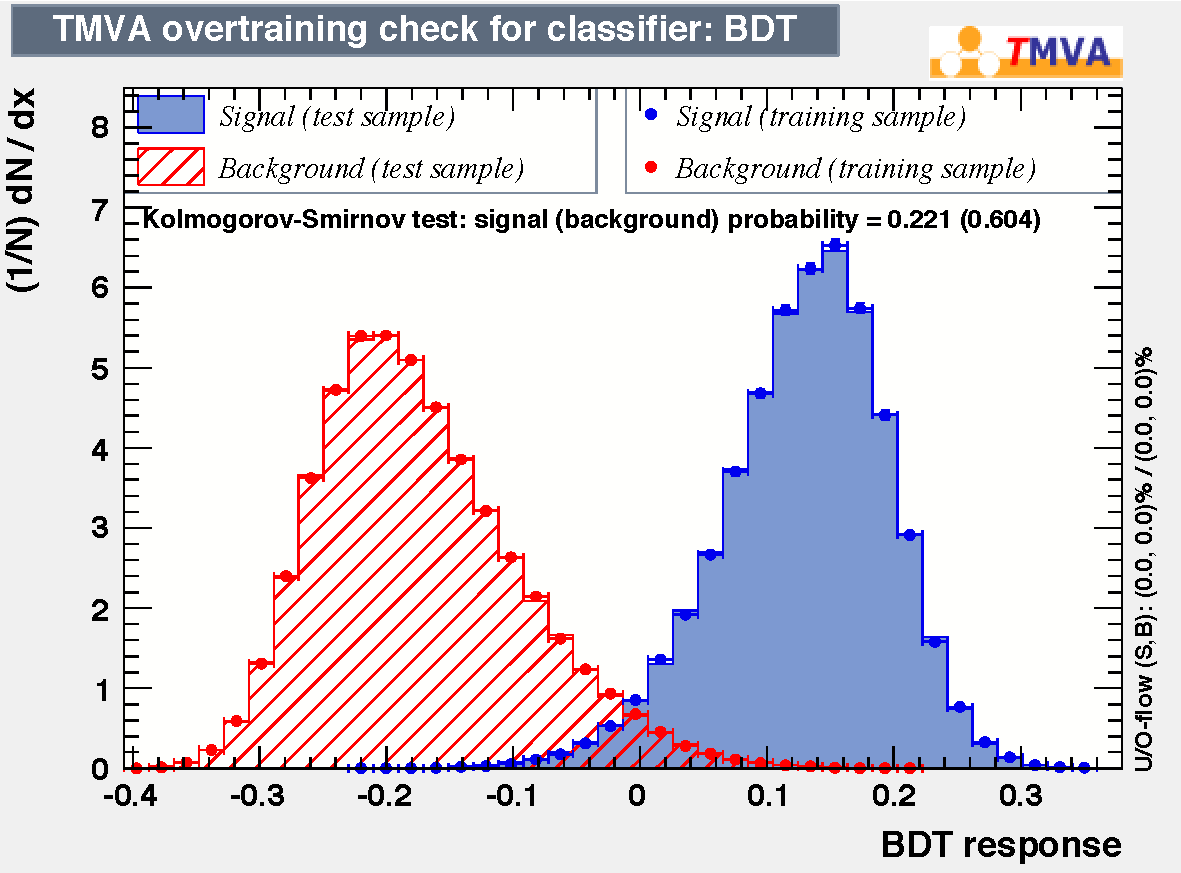
\includegraphics[width=0.7\textwidth]{06selection/figs/overtrain_BDT.pdf}
    \caption{Comparison of \ac{BDT} responses on the training and test sample.}
    \label{fig:BDTOVertraining}
\end{figure}
The agreement between the \ac{BDT} output distributions on the training and test samples is also checked with a Kolmogorov-Smirnov test~\cite{Bohm:389738} which gives \num{0.221} and \num{0.604} for the signal and background samples and thus indicates a good agreement.

\subsection{BDT selection optimisation}
\label{sec:BDTOpt}

To optimise the cut on the \ac{BDT} response the uncertainties on the \CP parameters \Sf and \Sfbar are used.
For the optimisation all preselection cuts, the vetoes for background from semileptonic decays and $\Lb\!\to\Lcbar\pip$ decays and the veto for wrongly associated \ac{PV}s are applied to the full dataset of both Run I.
To determine the uncertainty of \Sf and \Sfbar depending on the \ac{BDT} response the following strategy is adopted:
The \ac{BDT} output is scanned with a step size of \num{0.01} within a narrow range from \numrange{-0.15}{0.1} and with a step size of \num{0.05} in the outer regions.
For each cut on the \ac{BDT} response a fit to the invariant \Bz mass in the range \SIrange[per-mode=symbol]{5200}{5500}{\MeVcc} using the \emph{pion}-sample is performed.
This fit is used to determine \emph{sWeights}~\cite{Pivk:2004ty} and to obtain the mass shape which corresponds to the respective cut on the \ac{BDT} output.
Applying the \emph{sWeights} to other observables such as the decay time makes these distributions appear like signal-only~\cite{2009arXiv0905.0724X}.
Therefore, using \emph{sWeights} the tagging efficiencies, the shapes of the mistag distributions of the OS and SS tagging algorithms (more details on the flavour tagging can be found in \cref{ch:flavourtagging}) and the shape of the decay-time acceptance are obtained for the \enquote{signal} distributions.
The shape of the last is obtained in the same way as described in \cref{sec:acceptance}.
For each cut point then a single pseudoexperiment is performed: The invariant mass distribution is generated using the obtained signal and background yields and shapes from the mass fit, for the mistag and decay time distribution signal and background are both generated using the signal shapes.
The generated values for the \CP parameters are taken from simulation.
This pseudoexperiment sample is then fitted back: After determining \emph{sWeights} from a fit to the invariant \Bz mass distribution, a \CP fit to the decay time distribution is performed, where the flavour tagging calibration is assumed to be perfect.
In \cref{fig:BDTopt} the uncertainties on \Sf and \Sfbar are shown as a function of the \ac{BDT} response.
The final cut point is chosen at the right end of the plateau at \num{0.0}, to have as few background as possible while achieving the best possible sensitivity.
\begin{figure}[tbp]
    \centering
    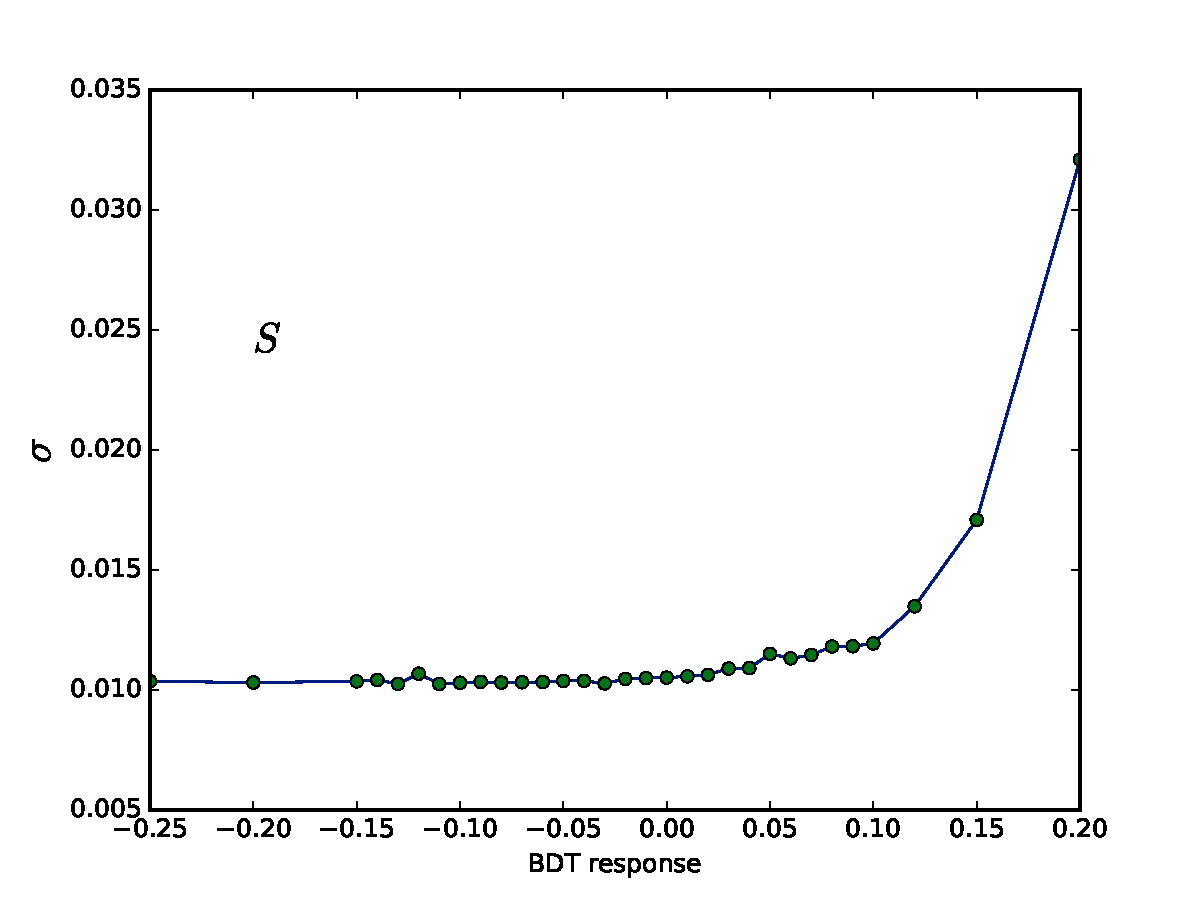
\includegraphics[width=0.49\textwidth]{06selection/figs/sensitiv_Sf.pdf}
    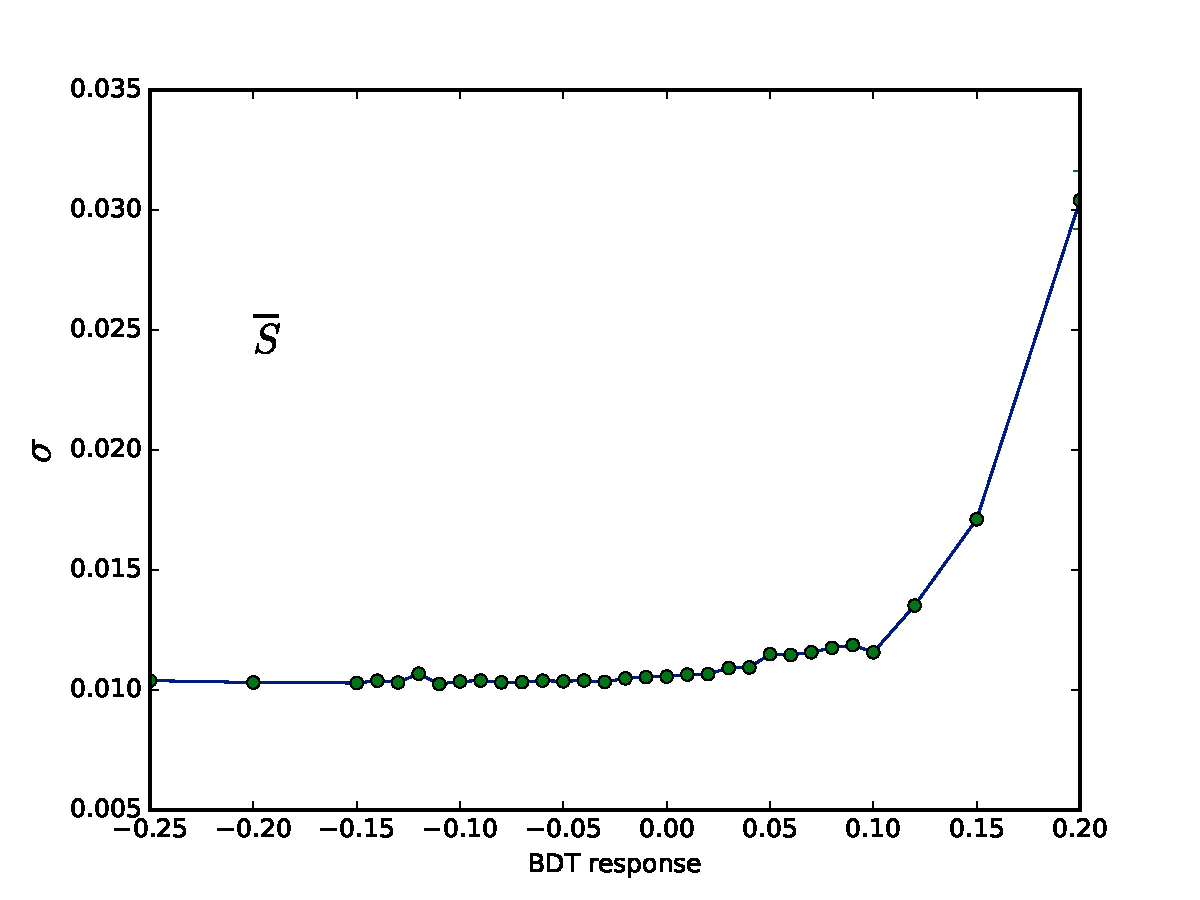
\includegraphics[width=0.49\textwidth]{06selection/figs/sensitiv_Sfbar.pdf}
    \caption{Uncertainty on \Sf (left) and \Sfbar (right) as a function of the \ac{BDT} response.}
    \label{fig:BDTopt}
\end{figure}

\subsection{Multiple Candidates}
\label{sec:MultCands}

In the stripping and trigger all used variables rely on the association of the \Bz candidate with the \ac{PV} to which the candidate has the smallest $\text{IP}\chi^2$, also denoted as best \ac{PV}.
To be consistent with this strategy for each event also the best \ac{PV} is chosen.
Events where the formerly best \ac{PV} is no longer present after the selection are removed.
Besides, events can contain more than one \Bz candidate.
After the stripping this is the case for \SI{9}{\percent} of the events and \SIrange{18}{20}{\percent} of the \Bz candidates share the same event.
This is reduced after applying the described selection steps, so that after selection only \SI{0.4}{\percent} of the events contain multiple candidates and \SI{0.8}{\percent} of the \Bz candidates share one event.
Following the proposal in \cite{Koppenburg:2017zsh} the remaining candidates are assumed to be equally likely signal candidates and one candidate per event is chosen at random.

\subsection{Selection Performance}
\label{sec:selectionPerformance}

The final selection performance is determined on the upper mass sideband with \mbox{$m_{\left[\Km\pip\pip\right]\pim}>\SI[per-mode=symbol]{5500}{\MeVcc}$} of the data and simulation based on the conditions of the \num{2012} data taking.
The corresponding signal efficiencies $\varepsilon_{\text{sig}}$ and background rejections $1-\varepsilon_{\text{bkg}}$ are given in \cref{tab:selPerform}.
\begin{table}[tbp]
	\centering
	\caption{Performances of all selection steps, where background refers to combinatorial background candidates.
	All efficiencies are calculated using the number of candidates after the previous selection step as \SI{100}{\percent}.
	The overall performance is given in the last row.}
	\begin{tabular}{ccc}
		\toprule
		Selection step						& $\varepsilon_{\text{sig}}$  & $1-\varepsilon_{\text{bkg}}$ \\
		\midrule
		preselection						& \SI{93.61\pm0.06}{\percent} & \SI{85.20\pm0.02}{\percent} \\
		\midrule
		$\Lz^\pm_\cquark$-veto				& \SI{93.48\pm0.06}{\percent} & \SI{9.85\pm0.03}{\percent} \\
		semileptonic veto					& \SI{98.96\pm0.03}{\percent} & \SI{7.66\pm0.03}{\percent} \\
		mass vetoes combined				& \SI{92.51\pm0.07}{\percent} & \SI{16.77\pm0.04}{\percent} \\
		\midrule
		wrongly associated \ac{PV}s veto	& \SI{97.75\pm0.04}{\percent} & \SI{15.81\pm0.04}{\percent} \\
		BDT selection						& \SI{83.63\pm0.10}{\percent} & \SI{97.18\pm0.01}{\percent} \\
		\midrule
		overall								& \SI{70.7\pm0.1}{\percent}   & \SI{99.911\pm0.002}{\percent} \\
		\bottomrule
	\end{tabular}
	\label{tab:selPerform}
\end{table}
The low background suppression of the vetoes is expected, as the vetoes aim to suppress specific backgrounds, but not the combinatorial background which is used to determine the given efficiencies.

Finally, the contamination with non resonant $\Bz\to\Kp\pim\pim\pip$ decays is determined, as such background would show the same structure as \BdToDpi candidates in the invariant $m_{\Kp\pim\pim\pip}$-distribution, but the \emph{weak} phase would be different.
In order to do this, two strategies are implemented, both using the datasample after applying all selection steps, except for the cut on the invariant \Dm-mass described in \cref{tab:preselection}:
For the first strategy the invariant \Dm-mass is plotted for candidates in a tight \Bz signal window from \SIrange[per-mode=symbol]{5240}{5320}{\MeVcc} as shown in \cref{fig:nonRes_Try1}.
\begin{figure}[tbp]
    \centering
    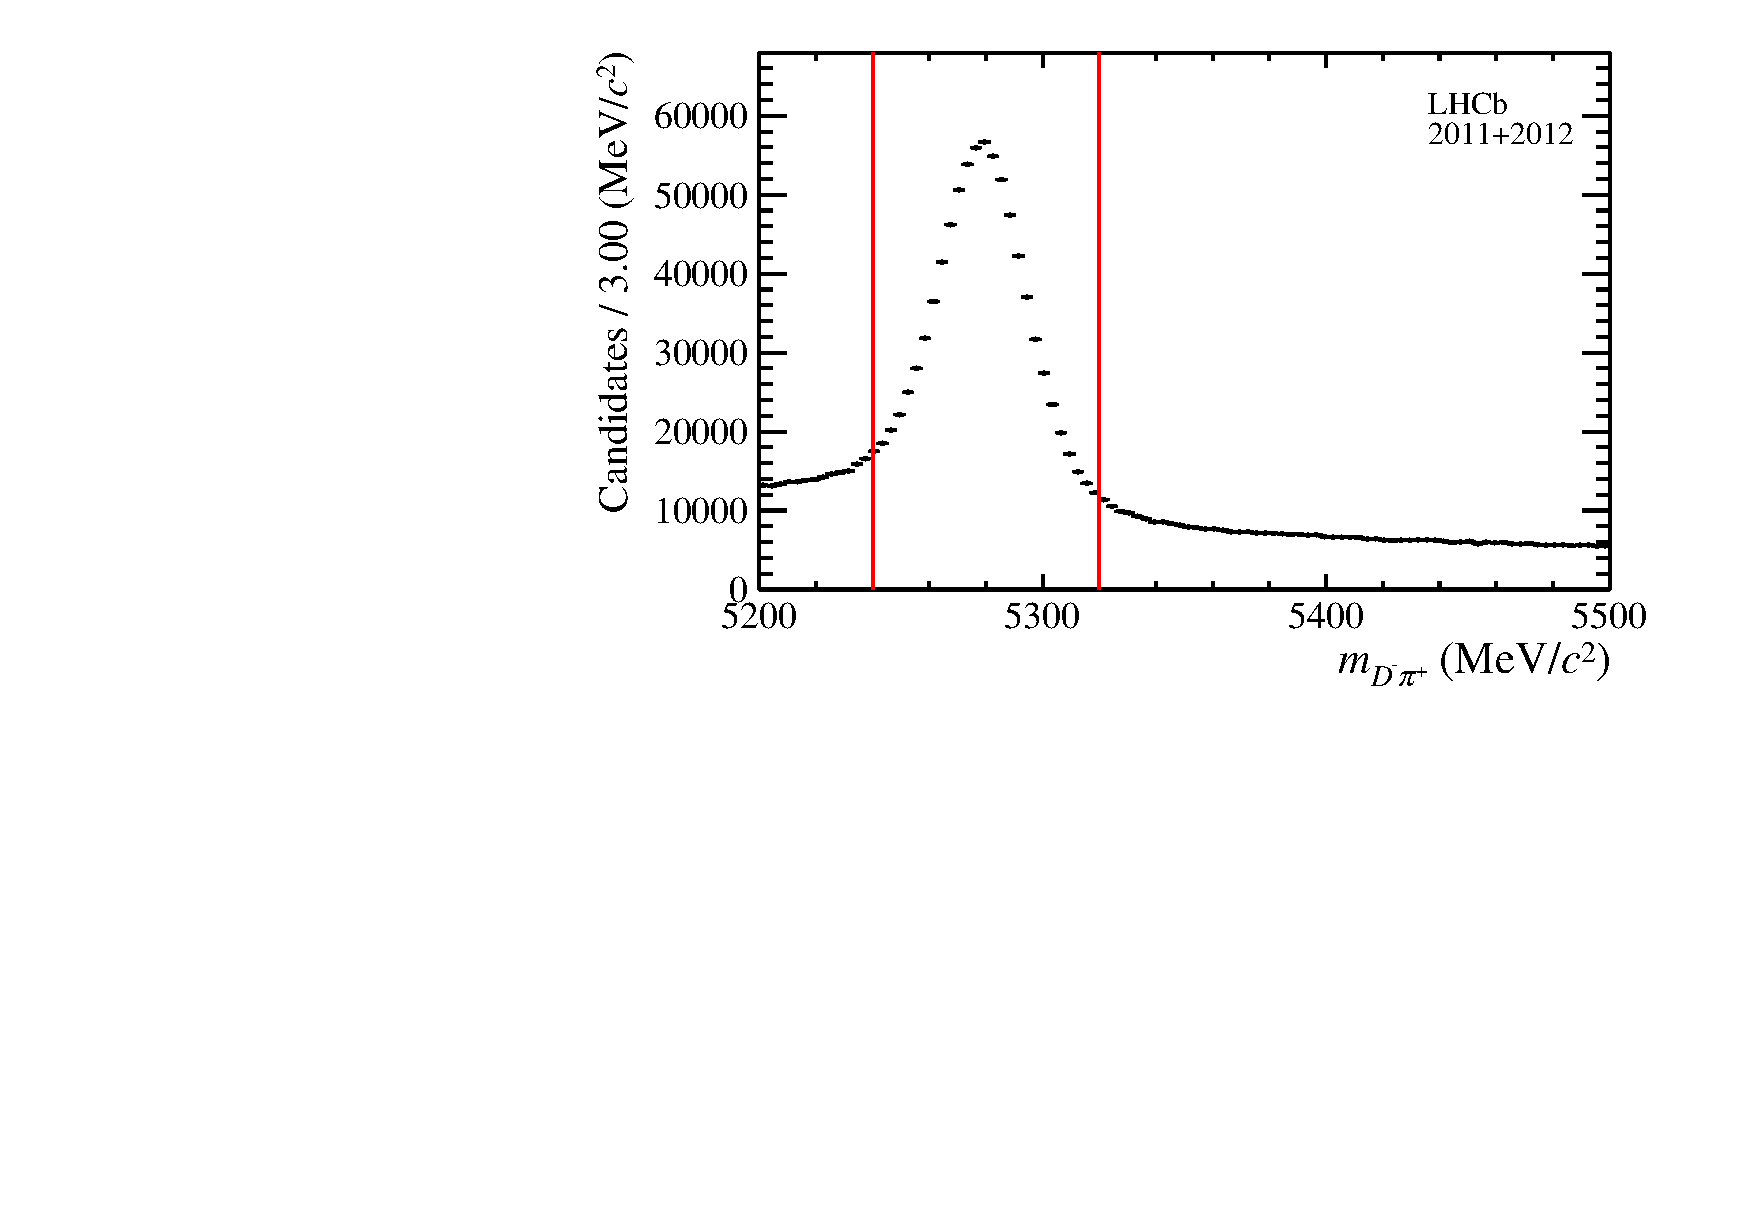
\includegraphics[width=0.49\textwidth]{06selection/figs/BmassCut.pdf}
    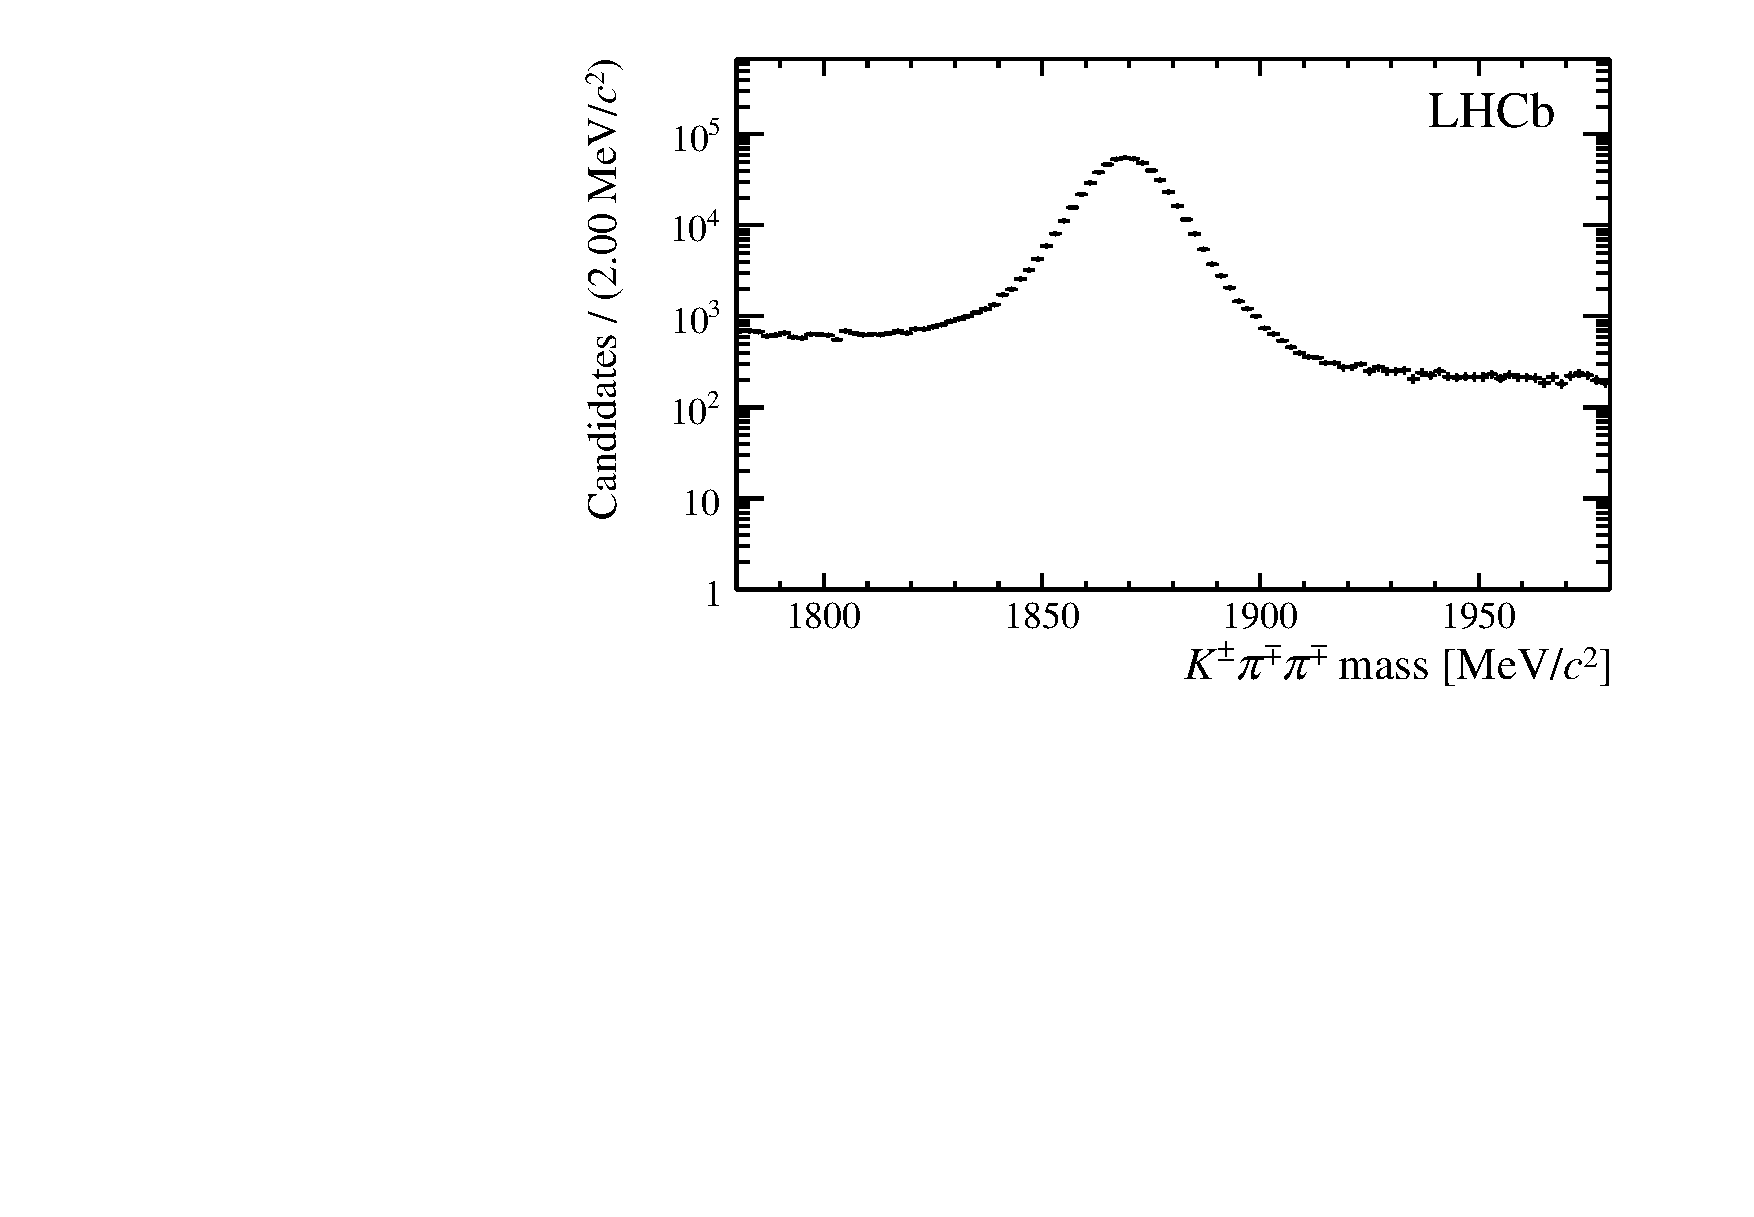
\includegraphics[width=0.49\textwidth]{06selection/figs/Resulting_Dmass.pdf}
    \caption{Left: Invariant \Bz-mass distribution with the selected signal region between the red vertical lines.
    Right: Resulting invariant \Dm-mass distribution.}
    \label{fig:nonRes_Try1}
\end{figure}
From the invariant \Dm-mass distribution the non-resonant contamination can be estimated to be roughly \SI{1}{\percent}.
In the second strategy a cut on the invariant \Dm-mass distribution removing the \Dm-peak is applied.
Then the invariant \Bz-mass without constraint on the \Dm-mass is inspected and a fit using an exponential to model the background and a gaussian with fixed shape to model the signal is performed to estimate the number of non-resonant $\Bz\!\to\Kp\pim\pim\pip$ candidates (see \cref{fig:nonRes_Try2}).
\begin{figure}[tbp]
    \centering
    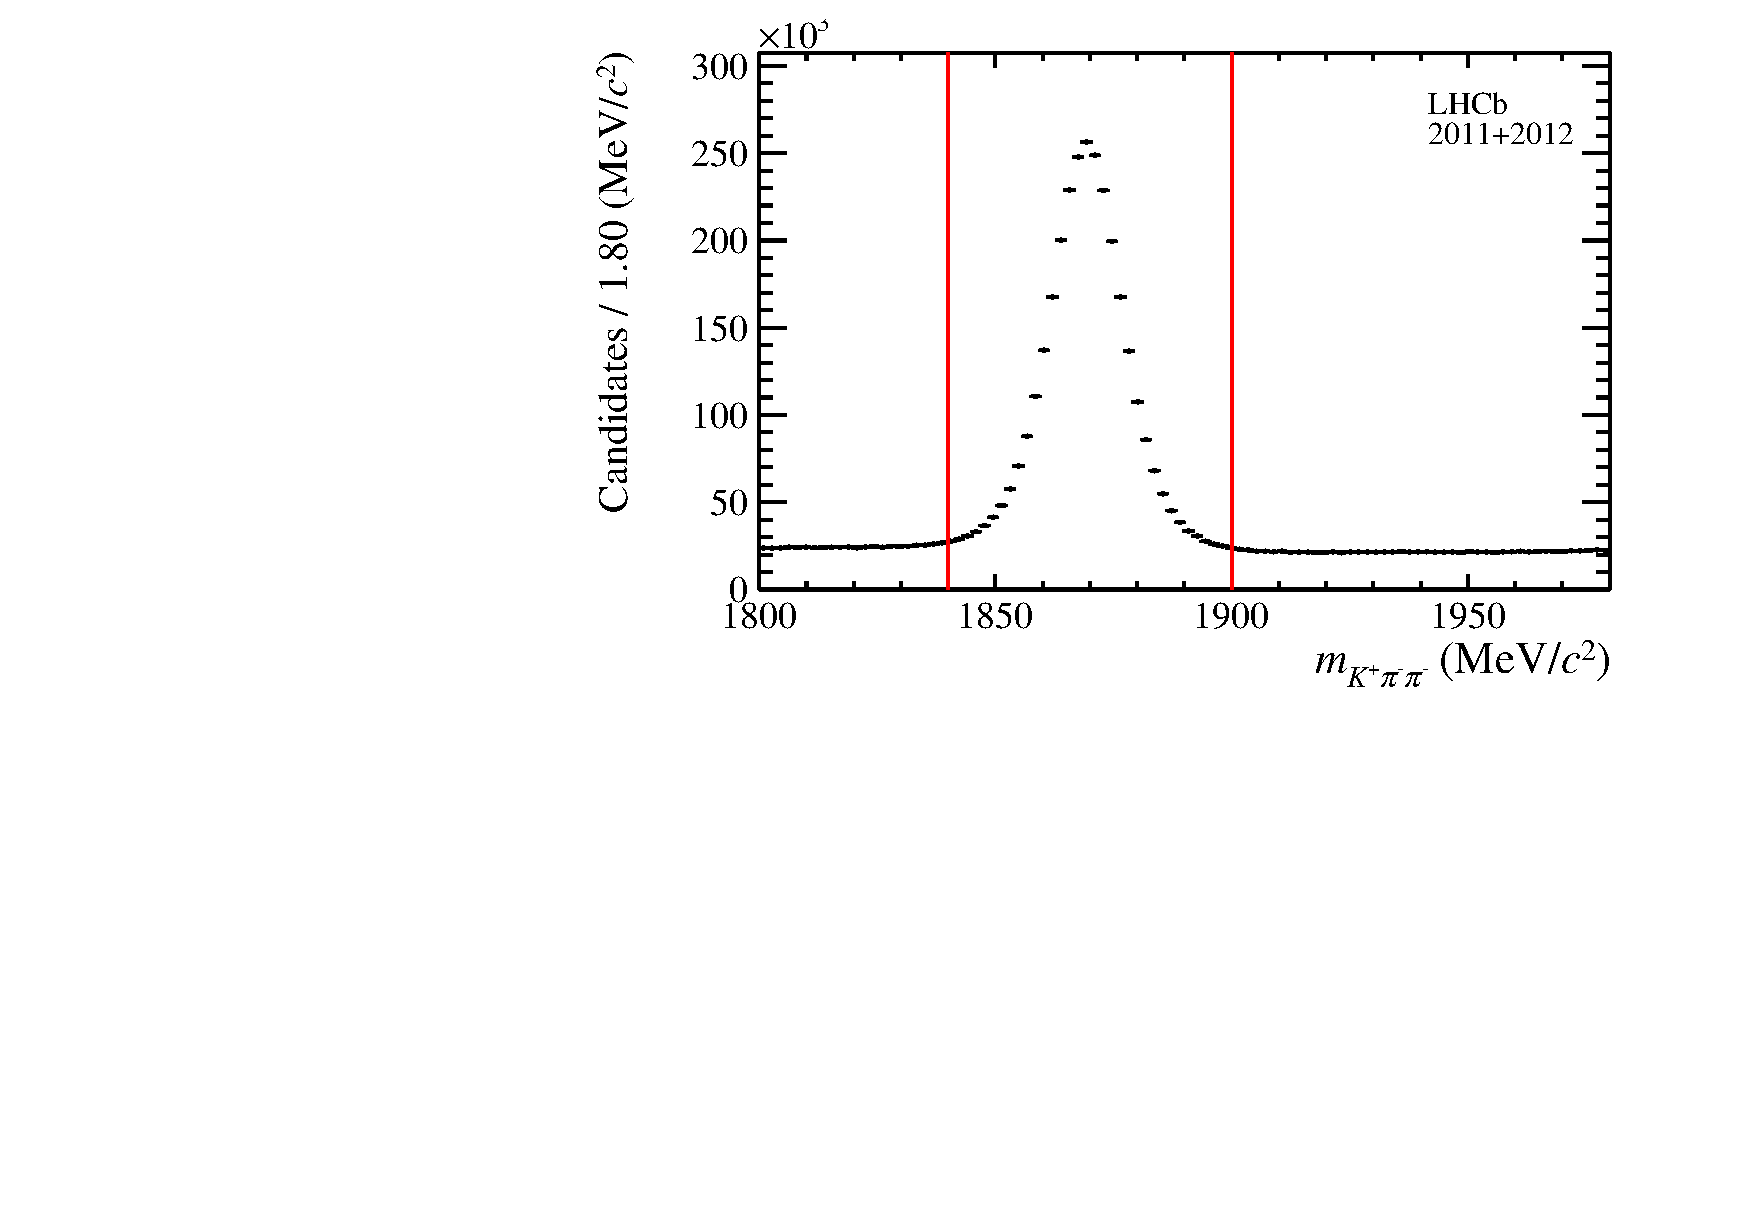
\includegraphics[width=0.49\textwidth]{06selection/figs/DmassCut.pdf}
    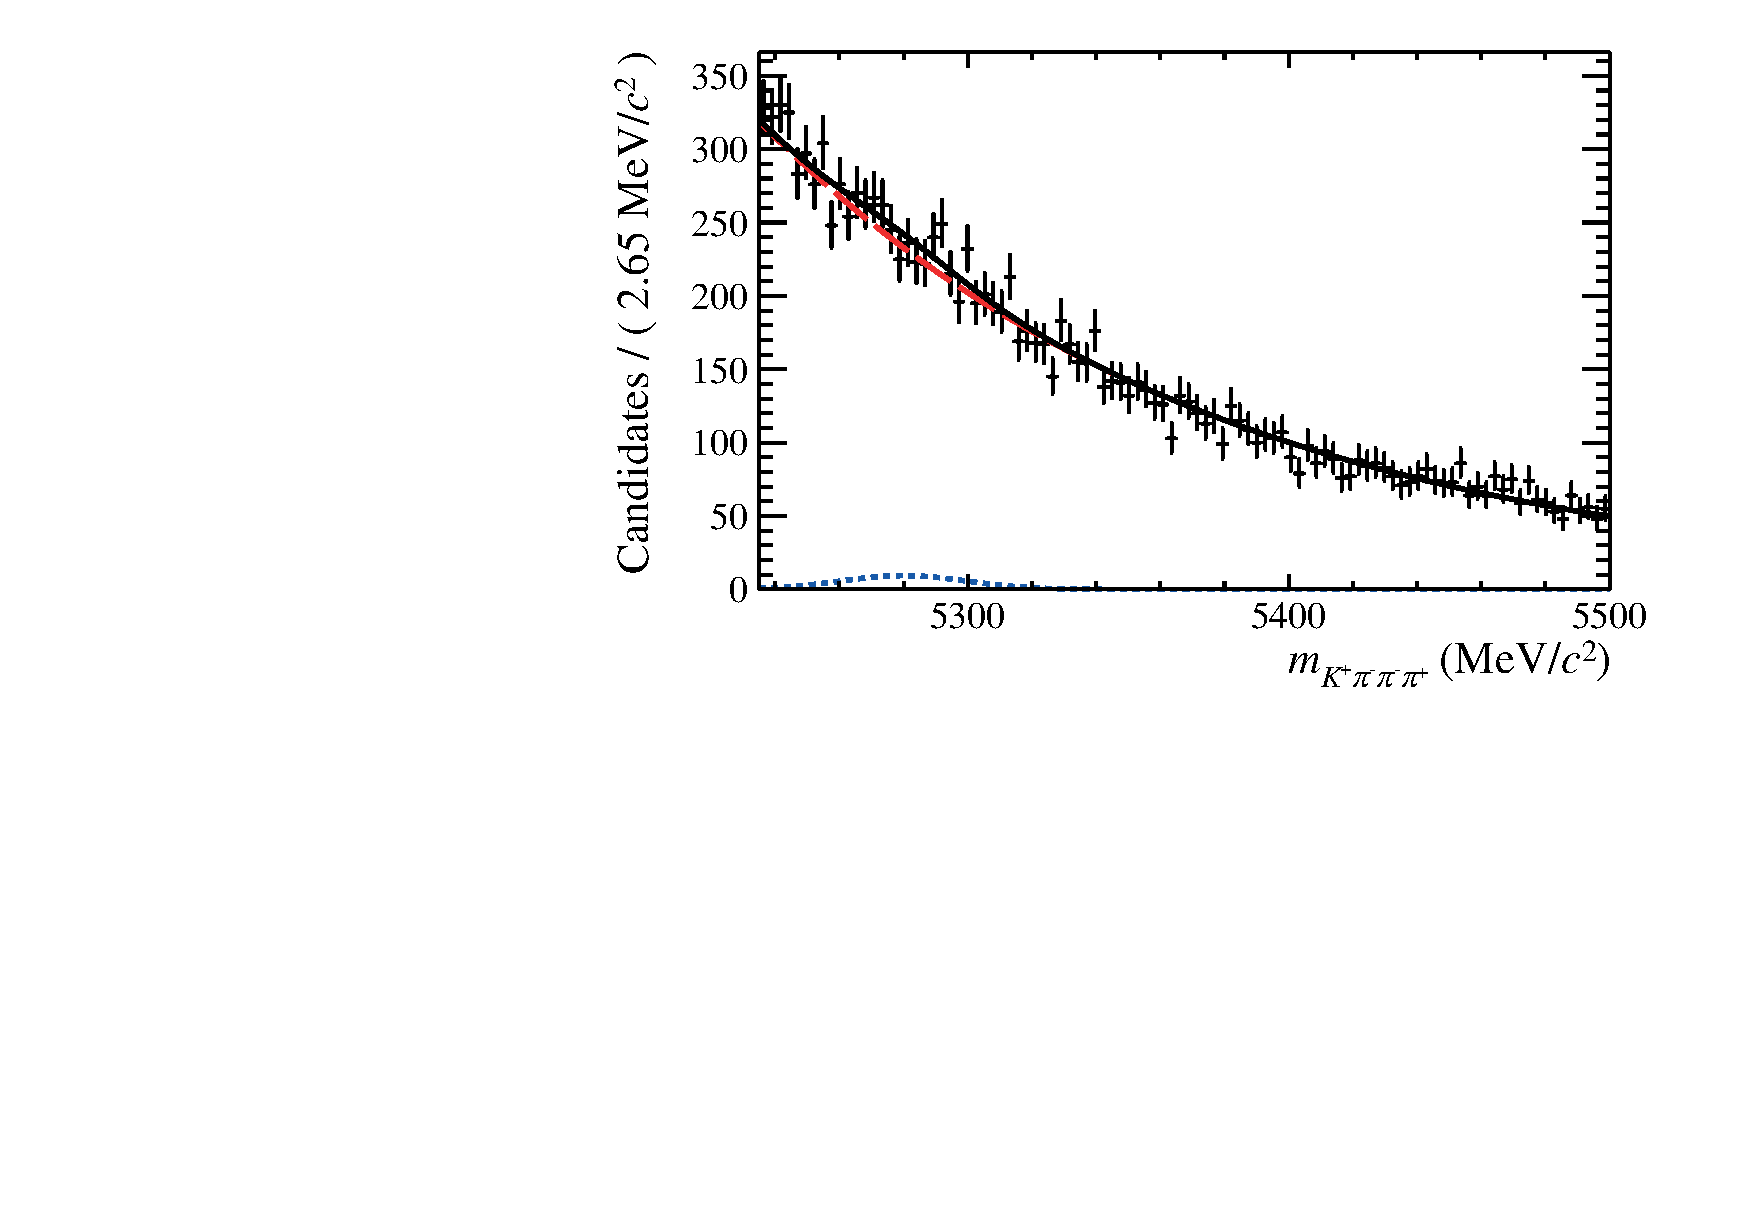
\includegraphics[width=0.49\textwidth]{06selection/figs/Resulting_Bmass.pdf}
    \caption{Left: Invariant \Dm-mass distribution with the excluded signal region between the red vertical lines.
    Right: Resulting invariant \Bz-mass distribution with the fit overlaid. The red dashed line describes the combinatorial background, the blue dotted line the signal component.}
    \label{fig:nonRes_Try2}
\end{figure}
This fit yields \num{645\pm242} signal candidates.
As both strategies do not show a significant amount of a non-resonant contamination of the sample, this is assumed to be negligible.
